\documentclass{llncs}

\usepackage{subfigure}
\usepackage{color}
\usepackage[usenames,dvipsnames]{xcolor}
\usepackage{graphicx}
\usepackage[numbers, sectionbib]{natbib}
\usepackage{tabularx}

\usepackage{anyfontsize}
\usepackage{fontspec}
\setmainfont{Times New Roman}

\usepackage{listings}
\lstnewenvironment{code}[1][]%
  {\minipage{0.9\linewidth} 
   \lstset{basicstyle=\ttfamily\footnotesize,frame=single,#1}}
  {\endminipage}

\definecolor{lightgray}{gray}{0.95}

\begin{document}

\title{Evaluating Open Information Extraction for Ontologization of a Thematic Domain}

\author{Gopala Krishna Koduri\inst{1} \and Siva Reddy Goli\inst{2} \and Bharat Ram Ambati\inst{2} \and Xavier Serra\inst{1}}
\institute{Music Technology Group, Universitat Pompeu Fabra, Barcelona, Spain \and
Institute for Language, Cognition and Computation, University of Edinburgh, UK \\
\email{gopala.koduri@upf.edu}
}

\maketitle

\begin{abstract}
In the past decade, domain-independent approaches to information extraction have paved way for its web-scale applications. Adapting them further to acquire knowledge from thematic domains can greatly reduce the need for manual knowledge engineering. This requires understanding how amenable the assertions extracted by such approaches are, to ontologization. To this extent, we propose a framework for a comparative evaluation of the open information extraction systems. The first part of the framework compares the volume of assertions along different dimensions with an aim to understand their coverage of the domain quantitatively. In the second part, the assertions are evaluated qualitatively by employing them in three of the fundamental tasks of ontologization: object identification, concept identification and semantic relation extraction. The combined observations lead to useful insights about not only the quality of the assertions, but also the nature of the information extraction approaches.
\end{abstract}

\section{Introduction}
\label{sec:intro}
The advent of the semantic web and the linked open data movements have not only resulted in a growing number of community-built structured data sources, but also catalyzed the development of domain-independent approaches for extracting information from unstructured text, further enriching them. Open information extraction (OIE) is one such paradigm that has emerged in the past decade, and has been used to extract assertions from unstructured data at web-scale with a considerable success [ref]. Until recently, domain-specific approaches to information extraction from text required manual knowledge engineering as a prerequisite [refs]. The OIE approaches, however, do not require a prespecified vocabulary and/or relation-specific input. Therefore, adapting them to information extraction from thematic domains would alleviate the need or manual knowledge engineering.

The process of channeling the assertions extracted from these approaches into a coherent knowledge-base itself poses certain challenges. There has been little work so far to identify and address such issues. In this paper, we propose a framework for a comparative evaluation of the open information extraction approaches. The first part of the framework compares the volume of extracted assertions across different aspects of a given domain with an aim to understand the coverage of the domain quantitatively. In the second part of the framework, the assertions are used in three fundamental tasks of ontologization: object identification, concept identification, and semantic relation extraction. The results from each task are validated against structured content in Wikipedia and/or are manually checked as necessary. The results from the two parts of the framework, when juxtaposed against each other, give us concrete insights into the differences between the performances and the nature of the approaches.

The remainder of the paper is organized as follows. In sec. xx,  an overview of the data we work with is presented, and in sec. xx, the OIE approaches that we chose to compare are discussed. In sec. xx, we present the framework with various quantitative and qualitative measures for analysing their performances on the tasks of relation extraction and ontologization, and demonstrate it using a thematic domain. Sec. xx concludes the paper with our observations and remarks.

\section{Open Information Extraction}
\label{sec:oie}
Information extraction is the task of obtaining a set of assertions from the natural language text, featuring the entities and the relations of the corresponding domain. The approaches are diverse ranging from those which learn from the labeled training samples for the desired set of target relations, to those which operate in an unsupervised manner. An easy access to large volume of unstructured text on the web has necessitated approaches that scale appropriately to take advantage of this data. Open information extraction is one such paradigm, which aims to extract the assertions from voluminous data without requiring a pre-specified vocabulary or labeled data for relations [refs].

\subsection{ReVerb \& OpenIE 4.0}
For demonstrating our evaluation framework, we choose two state-of-the-art OIE systems: ReVerb and OpenIE 4.0, which are shown to have outperformed the earlier systems such as TextRunner [ref], $woe^{pos}$ and $woe^{parse}$ [ref]. ReVerb addresses the issue of incoherent and uninformative extractions found with the former approaches, by using few syntactic and lexical constraints [ref]. OLLIE is a successor of ReVerb, and includes the noun-mediated relations which are not handled by the latter. It also incorporates the context of the assertions in the form n-ary relations [ref]. OpenIE 4.0 employs a similar methodology to that of OLLIE, to retrieve assertions by semantic role labeling, also known as shallow semantic parsing.

\subsection{Semantic parsing}
On the other hand, deep semantic parsing is an active research topic in the natural language processing (NLP) community, which aims to obtain a complete logical form of a given sentence. It facilitates applications such as question-answering systems, and further has several direct implications for OIE as it is domain-independent and is shown to be web-scalable [refs]. To our knowledge, there is no existing literature that compares it with the likes of ReVerb and OpenIE 4.0. We therefore built an information extraction wrapper around a state-of-the-art semantic parser, to be compared with the selected OIE approaches. What follows is a brief description of this system.

We use Combinatory Categorial Grammar (CCG, Steedman 2000) as our grammatical framework to parse natural language sentences to logical representation. CCG is known for its transparency between syntax and semantics, i.e. given the syntactic structure (CCG derivation) of a sentence, a semantic (logical) representation can be built deterministically from its derivation. Each word in a sentence is first assigned a CCG category based on its context. Each category represents the syntactic constraints that the word has to satisfy. For example, in Figure.~\ref{fig:ccg_sample}, the word \textit{plays} is assigned a syntactic category $(S\backslash NP)/NP$ implying that \textit{plays} take a noun ($NP$) argument on its right, and a noun argument ($NP$) on its left to form a sentence ($S$). An equivalent semantic category in terms of a lambda function is constructed from the syntactic category, here $\lambda x. \lambda y. \mathrm{plays}(subj,~y) \wedge \mathrm{plays}(obj,~x)$ with \textit{plays} representing the predicate, $x$ and $y$ representing the object (guitar) and subject (John) arguments. CCG defines a set of combinators using which the adjacent categories combine to form syntactic categories of larger text units like phrases (\textit{e.g:} plays guitar), from there on leading to parsing a whole sentence. Correspondingly, the lambda functions of the categories compose, eventually leading to semantic representation of the sentence. The advantage with CCG is that the complexity of obtaining a logical representation of the sentence is simplified into the task of assigning categories to words. We use a modified version of Boxer (Bos et al. 2004) to further convert our sentences of interest to binary assertions of the form <argument 1, relation phrase, argument 2>.
\begin{figure}[!t]
\centering
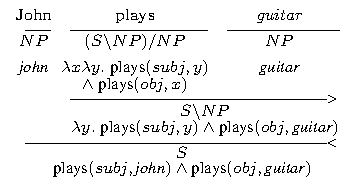
\includegraphics[width=0.6\linewidth]{figures/ccg_sample.pdf}
\caption{An example showing the sentence `John plays guitar', parsed using CCG.}
\label{fig:ccg_sample}
\end{figure}

\section{Data}
\label{sec:data}
A major challenge in developing technologies for the exploration and the navigation of music repertoires from around the world, lies in obtaining and using their cultural context. The vocabulary used for describing and relating the entities (musical concepts, roles of people involved etc) differs to a great extent from music to music. Most commercial platforms have a limited view of such context, resulting in poor navigation and exploration systems that fail to address the cultural diversity of the world.  Within the music information research community, there is a growing interest for developing culture-aware approaches to address this problem [ref compmusic]. Such approaches are diverse in terms of the data they work with (audio, metadata and contextual-data) and methodologies they employ [ref: mires]. 

However, to our knowledge, there are no major attempts that use text, arguably the largest openly available data source. As a first step in this direction, we choose to demonstrate our framework in the music domain. Indian art music traditions: Carnatic and Hindustani, have a very distinct character, especially when compared to the popular music styles that drive the music market worldwide [ref]. The terminology and the structuring of the knowledge in these music traditions differs substantially from what people are accustomed to, on most commercial platforms. Therefore, they make a suitable yet challenging thematic domain to analyze the quality of the assertions for ontologization. 

Our data consists of the plain text obtained from 618, 697 Wikipedia pages corresponding to the Carnatic and Hindustani music traditions, respectively, after removing the tables, listings, figures, infoboxes and other structured content. Text from each page is tokenized to sentences, which are further filtered using the following constraints: a minimum number of 3 words and a maximum of 21 words per sentence, with each word not exceeding 30 characters in length. These constraints are empirically found to greatly reduce the number of malformed and highly complex sentences.

We observed that a majority of the sentences featured pronouns. The resulting assertions only partially contribute to ontologization. For instance, consider the sentence `She is a Composer'. The resulting assertion would be <She, is a, Composer>. With a few more of such sentences, it is possible to learn that there exists a semantic category called \textit{composer}. However, such assertions are helpless in identifying objects of the corresponding semantic category. Therefore, the pronouns in the text from each page are resolved using [ref]. There were a few false assertions as a result. However, there is a substantial rise in the recall of the entities in the domain. Table. xx list the total number of sentences, and the number of extractions from each of the OIE systems.
%TODO we can add the number of He/she pronouns resolved to put it in perspective.

\begin{table}
 \begin{center}
 \begin{tabularx}{0.9\textwidth}{X X X X X}
 \noalign{\hrule height 1.1pt}
  \textbf{Music} & \textbf{\#Sentences} & \textbf{\#ReVerb} & \textbf{\#OpenIE 4.0} & \textbf{\#Sem. Parsing}\\
  \hline
  Carnatic  & 10284 & 9844 & 15013 & 19241 \\
  Hindustani  & 10724 & 9944 & 15777 & 18496 \\
 \noalign{\hrule height 1.1pt}
 \end{tabularx}
\end{center}
\caption{The number of sentences for each music, and the number of extractions using different OIE systems.} 
\label{tab:data}
\end{table}

\section{Evaluation framework}
\label{sec:framework}
In the information extraction literature, comparing different approaches by their performances on a set of labelled sentences or by employing human judges, is a common practise [refs]. Our goal, however, is to evaluate them by the usefulness of the assertions extracted. We quantify this using a series of tasks that help in understanding the coverage of the entities and the relations of a given domain in the extracted assertions, quantitatively and qualitatively.  The tasks discussed in the first part of the evaluation comparing the volume of the assertions. while in the second part, we validate to what extent the assertions yield to be structured. We then juxtapose and compare the results from both parts of the evaluation.

\subsection{Quantitative assessment}
We study the distribution of the extracted assertions across four different aspects to gain an insight into their coverage of the domain with respect to each of them: \textbf{sentences}, \textbf{objects}, \textbf{relation types} and \textbf{concepts}. For the purpose of analyses discussed in this section, the first argument in the assertion is taken for an object, and the second argument of assertions featuring a subsumption relational phrase (eg: is a, be etc..) is taken for a concept.

Observations from the distribution of the extractions across sentences give a crude perspective of the modularity of the information extraction approach, which is its ability to identify multiple, distinct relations from a given sentence. The distribution of extractions across the objects allows us to gain an overview of the scope of the extracted relations in identifying the entities in the given domain as well as in describing a given entity. The distribution of extractions across relation types allows us to understand the relevance and coverage of an identified relation-type in the domain. 

As we will see, a large majority of the assertions from all the OIE systems correspond to the subsumption relation type, often outnumbering the other relation types by orders of magnitude. Therefore, it is important to further analyze this relation type. These relations mainly inform us about the semantic category membership of the entities. Hence, they assume importance for ontologization as they are resourceful in defining the taxonomy of the given domain. The distribution of extractions per class would reveal to what extent the assertions actually carry the required information.

\subsection{Qualitative assessment}
The tasks discussed in this section are complementary to those presented in the former, validating whether the quantitative observations correlate with the performances of OIE approaches on various tasks in ontologization. For this, we consider the three fundamental tasks of ontologization: object identification, concept identification and semantic relation extraction [refs]. 

\subsubsection{Concept identification.} It is the task of identifying the semantic categories in the domain. The second argument from all the assertions featuring the subsumption relation type are collected. They are disambiguated based on their spellings, mostly automatically using string matching algorithms with minimal manual intervention where necessary. The resulting arguments are taken to be concepts in the taxonomy of the given domain. We compare the coverage of this set of concepts against the ontologies manually built for each of the Carnatic and Hindustani music.

\subsubsection{Object identification.} It concerns with finding the entities of the given domain and assigning a semantic category to them. The set of first arguments from all the assertions are considered as candidates for being objects in the domain. A list of titles of the Wikpedia pages in the domain along with the categories each page belong to, is acquired.  The page titles correspond to objects, and the categories are manually mapped to concepts in our ontology. This constitutes the reference with which we compare the coverage of objects identified using the assertions from each of the OIE approaches.

For evaluating the first part of object identification, i.e., finding the entities of the given domain, we measure the overlap between the candidate objects from each approach with the reference set. The second part, semantic category assignment, is evaluated using two methods. In the first method, we manually build a set of rules using subsumption relation type for each semantic category. The objects satisfying the rules for a given semantic category are assigned to it. The second method takes advantage of the full spectrum of relation-types extracted. Each semantic category is bootstrapped using a seedset of objects belonging to it.

%TODO: write about the bootstrapping approach.

\subsubsection{Semantic relation extraction.} It refers to the relation types other than those which convey concept hierarchies. The relation shown in Figure. xx is one such example, where the relation \textit{plays} connects \textit{person} and \textit{musical instrument} semantic categories. We formulate two measures  to compare the OIE approaches in this task: \textit{breadth} and \textit{depth} of relation types. \textit{Breadth} corresponds to the number of valid relation types identified for each semantic category, and the \textit{depth} corresponds to the number of valid assertions for a given relation type.

\section{Results and discussion}
\subsection{Quantitative assessment}
\begin{figure}
\label{fig:quant-sentences}
\begin{center}
        \subfigure[][Carnatic music]{%
		 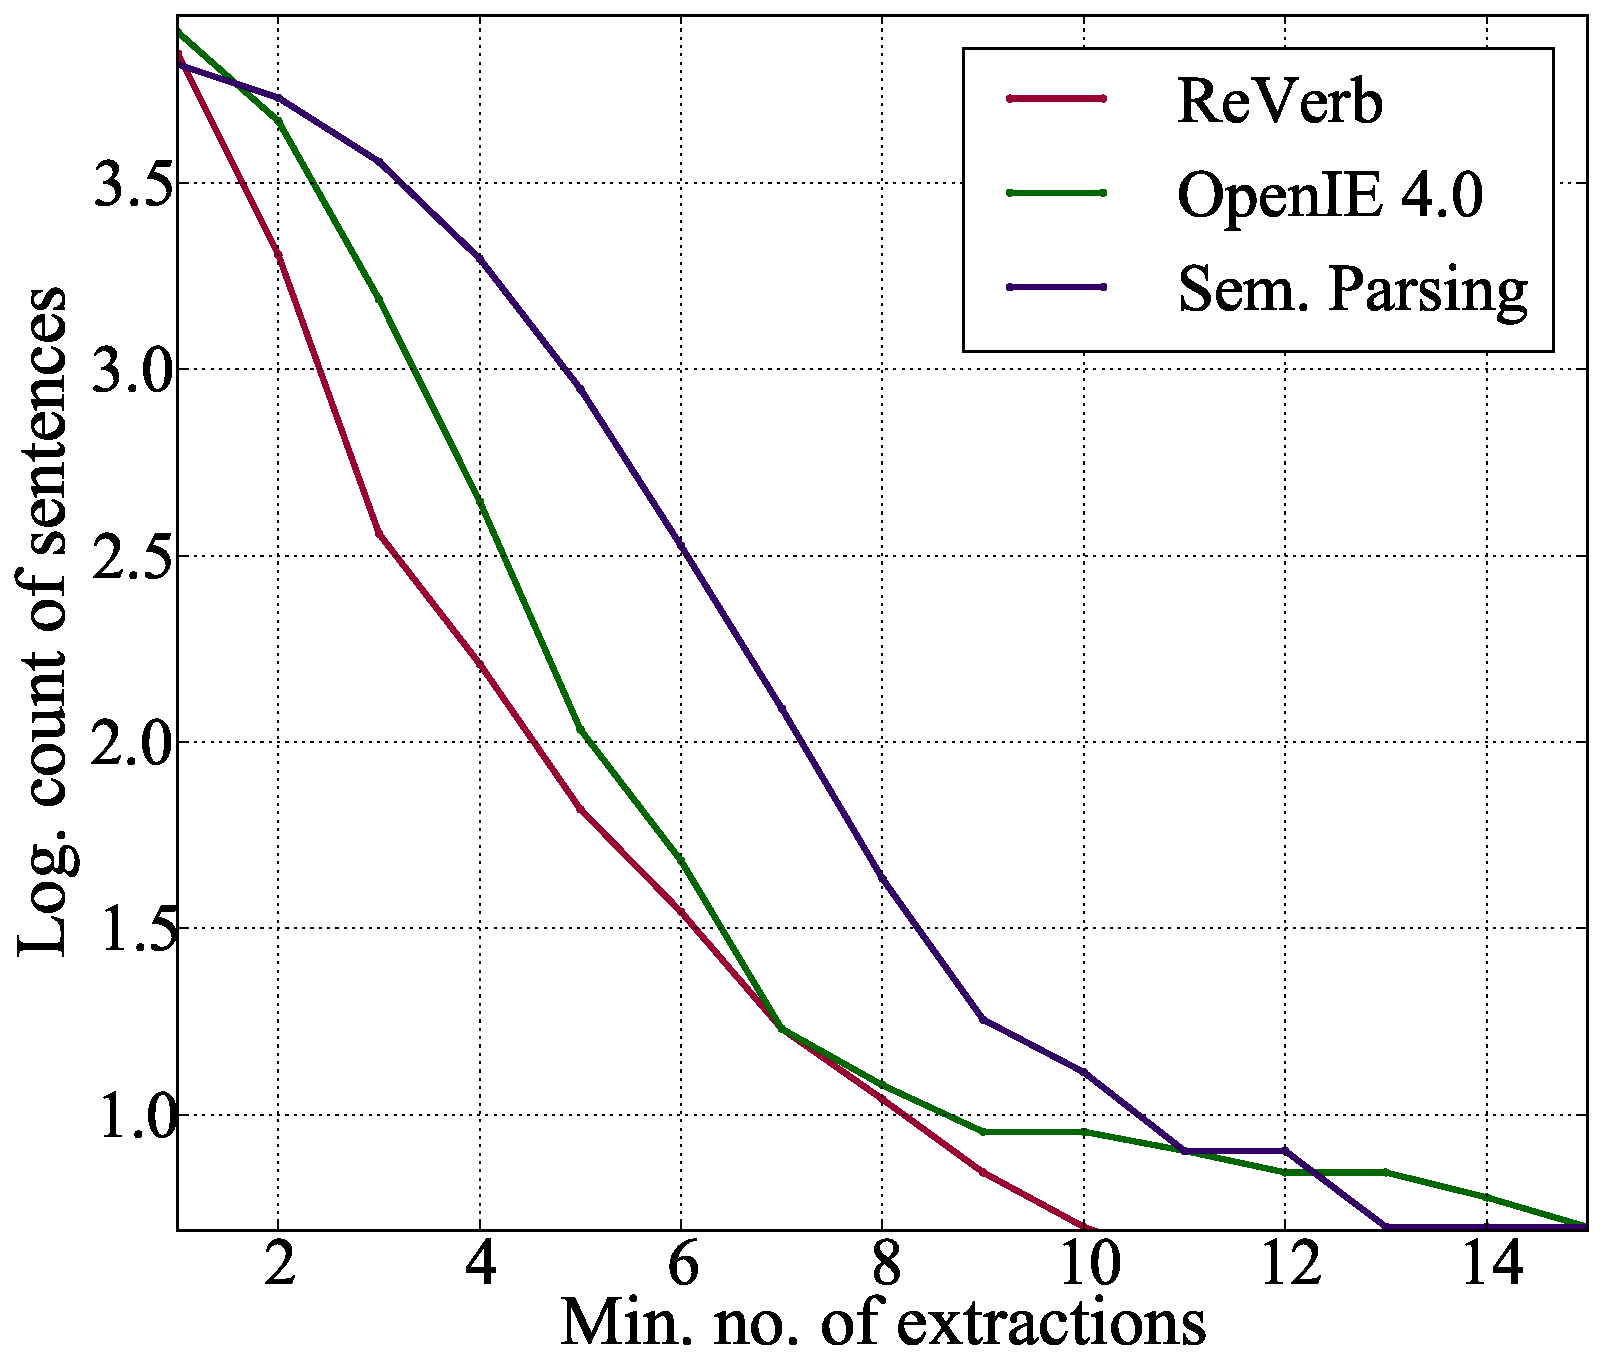
\includegraphics[width=0.45\linewidth]{../data/results/quantitative/carnatic_music/extrations-per-sentence.pdf}
		 \label{fig:quant-sentences-carnatic}
        }% 
        \qquad
        \subfigure[][Hindustani music]{%
		 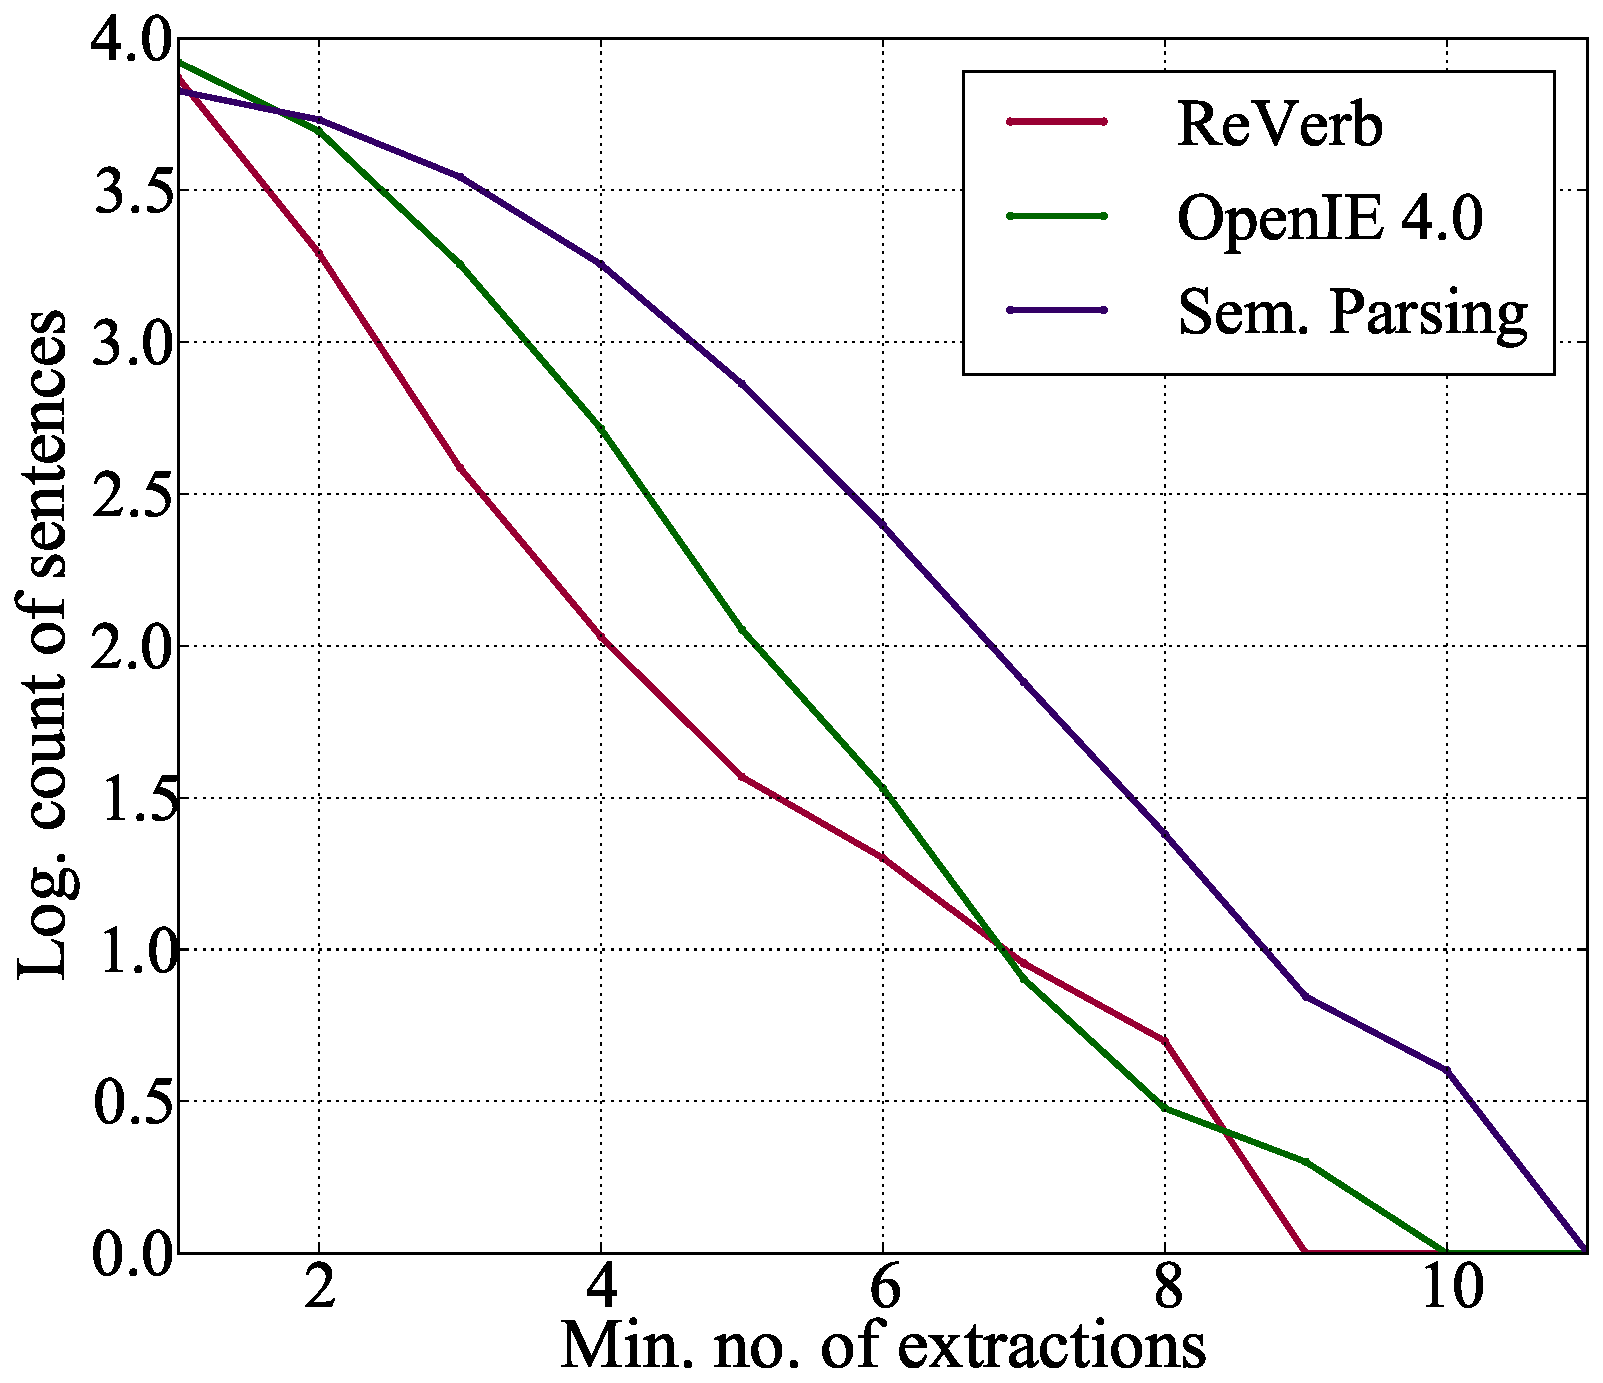
\includegraphics[width=0.45\linewidth]{../data/results/quantitative/hindustani_music/extrations-per-sentence.pdf}
		 \label{fig:quant-sentences-hindustani}
        }%
\end{center}
\caption{Distribution of number of extracted assertions using each of the approaches, per sentence.}
\end{figure}

\begin{figure}
\label{fig:quant-object}
\begin{center}
        \subfigure[][Carnatic music]{%
		 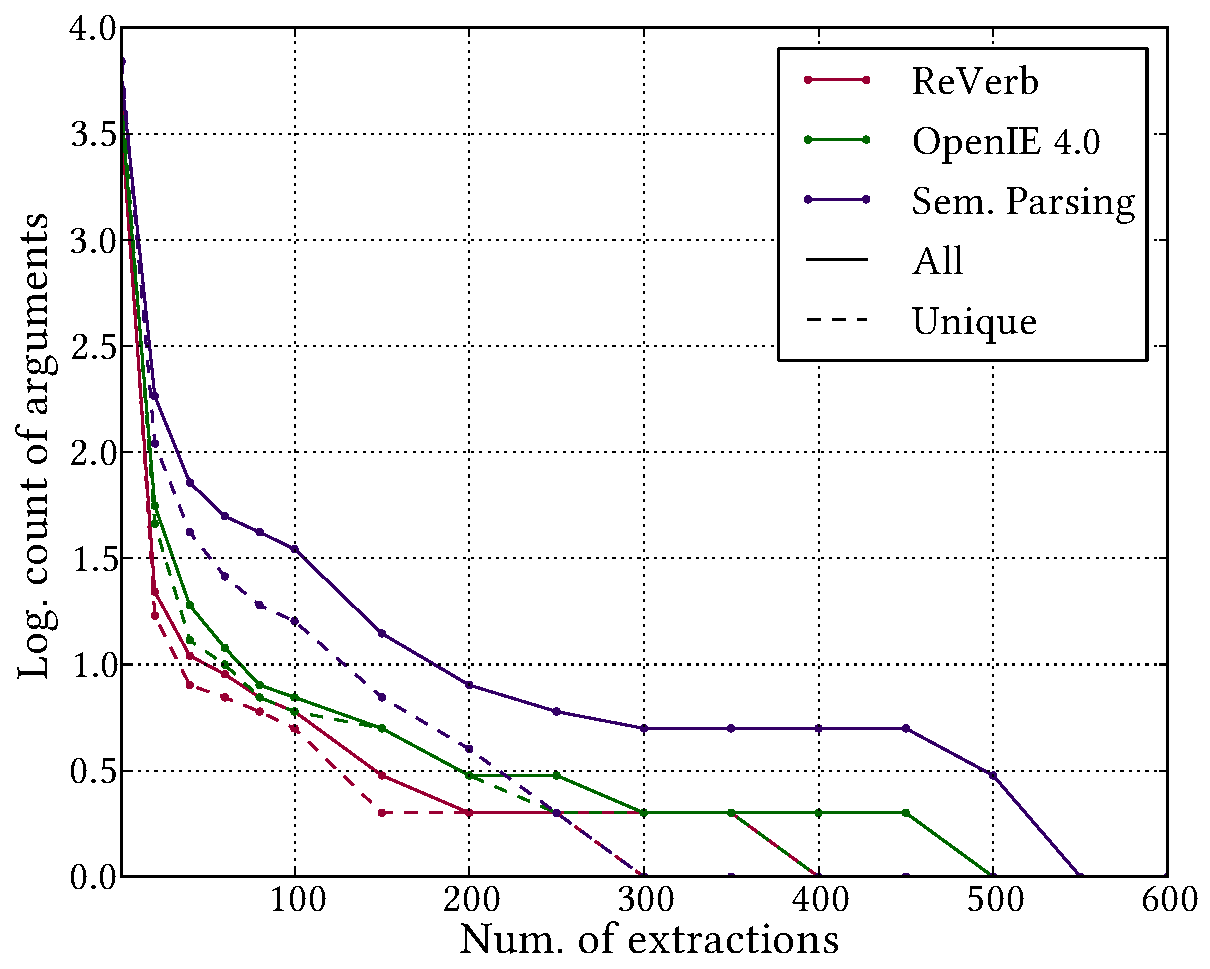
\includegraphics[width=0.45\linewidth]{../data/results/quantitative/carnatic_music/extrations-per-argument.pdf}
		 \label{fig:quant-object-carnatic}
        }% 
        \qquad
        \subfigure[][Hindustani music]{%
		 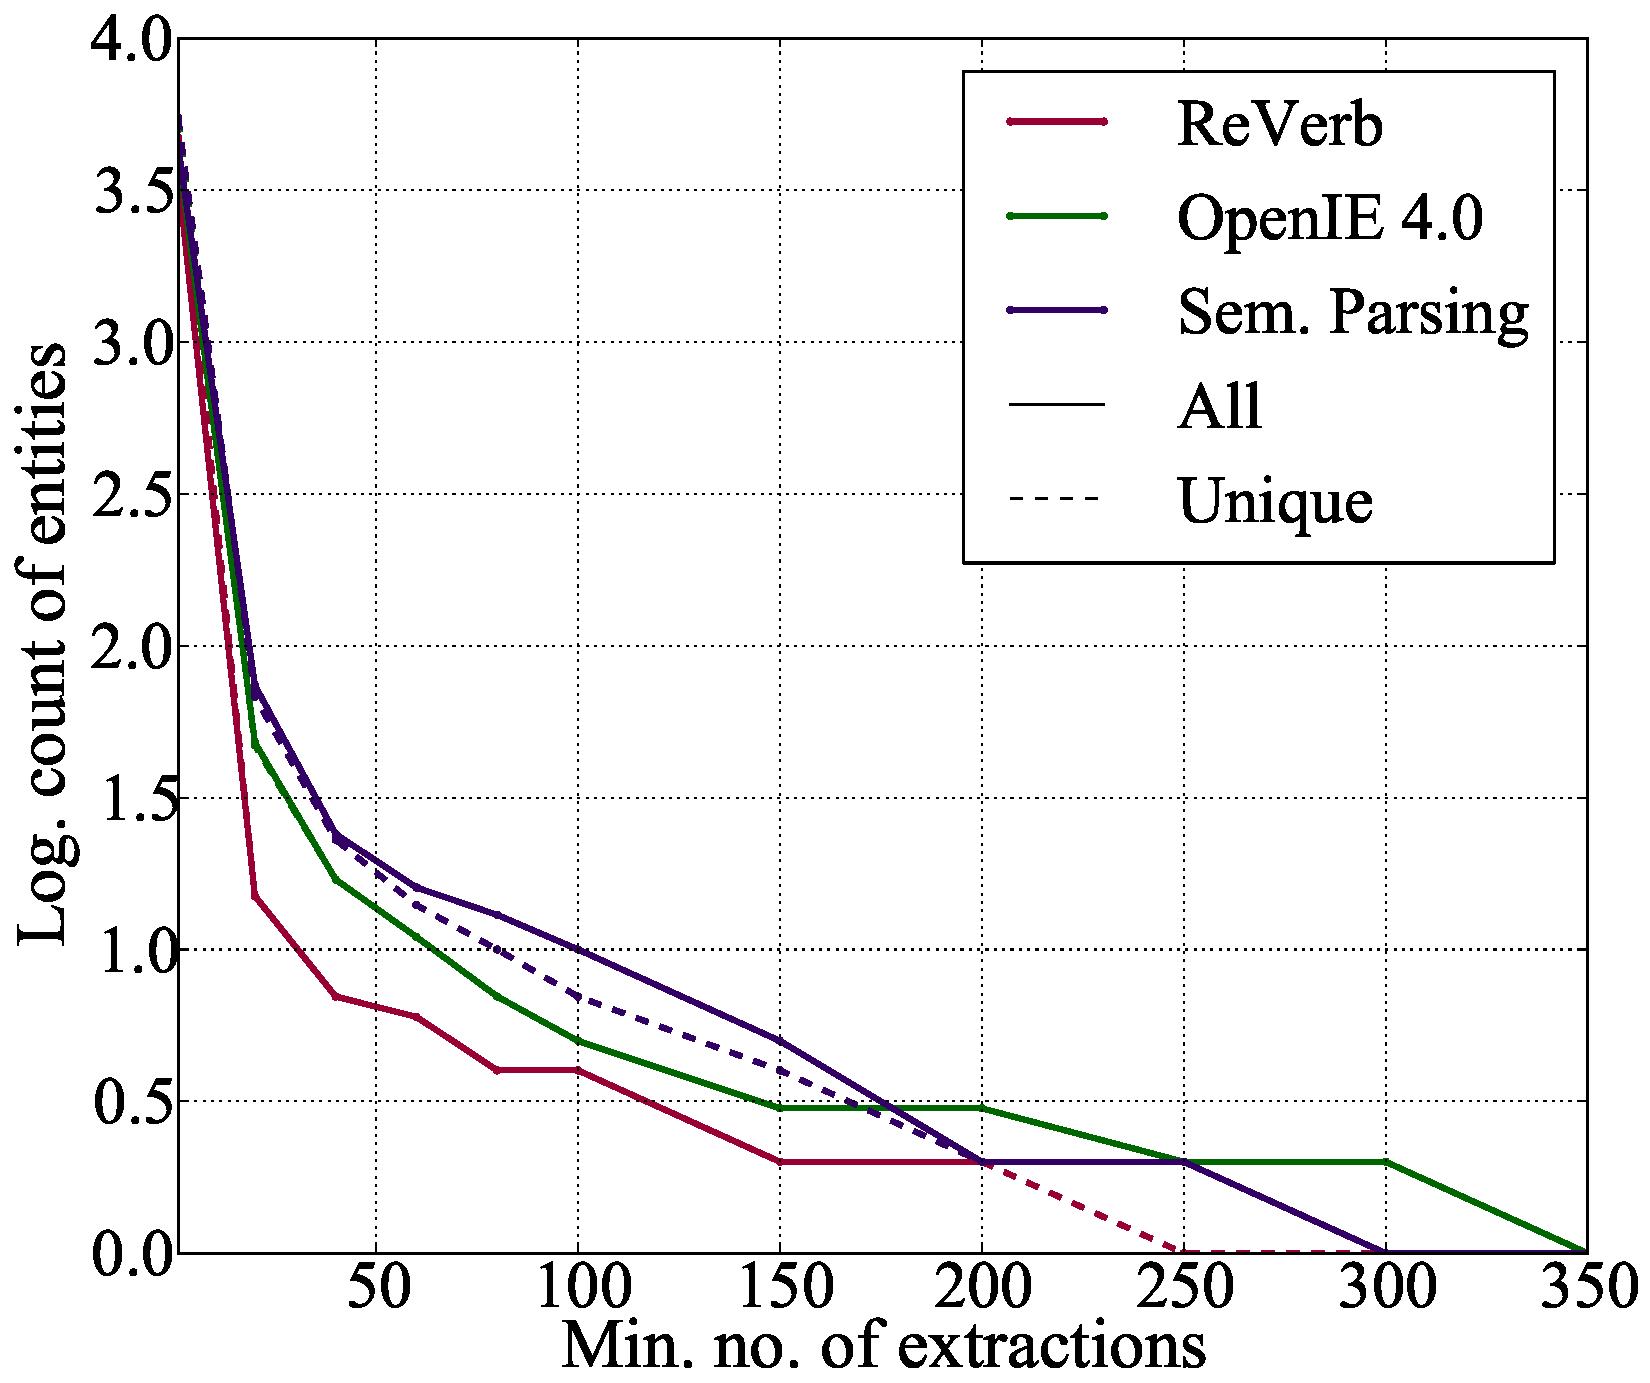
\includegraphics[width=0.45\linewidth]{../data/results/quantitative/hindustani_music/extrations-per-argument.pdf}
		 \label{fig:quant-object-hindustani}
        }%
\end{center}
\caption{Distribution of number of extracted assertions using each of the approaches, per object.}
\end{figure}

\begin{figure}
\label{fig:quant-reltype}
\begin{center}
        \subfigure[][Carnatic music]{%
		 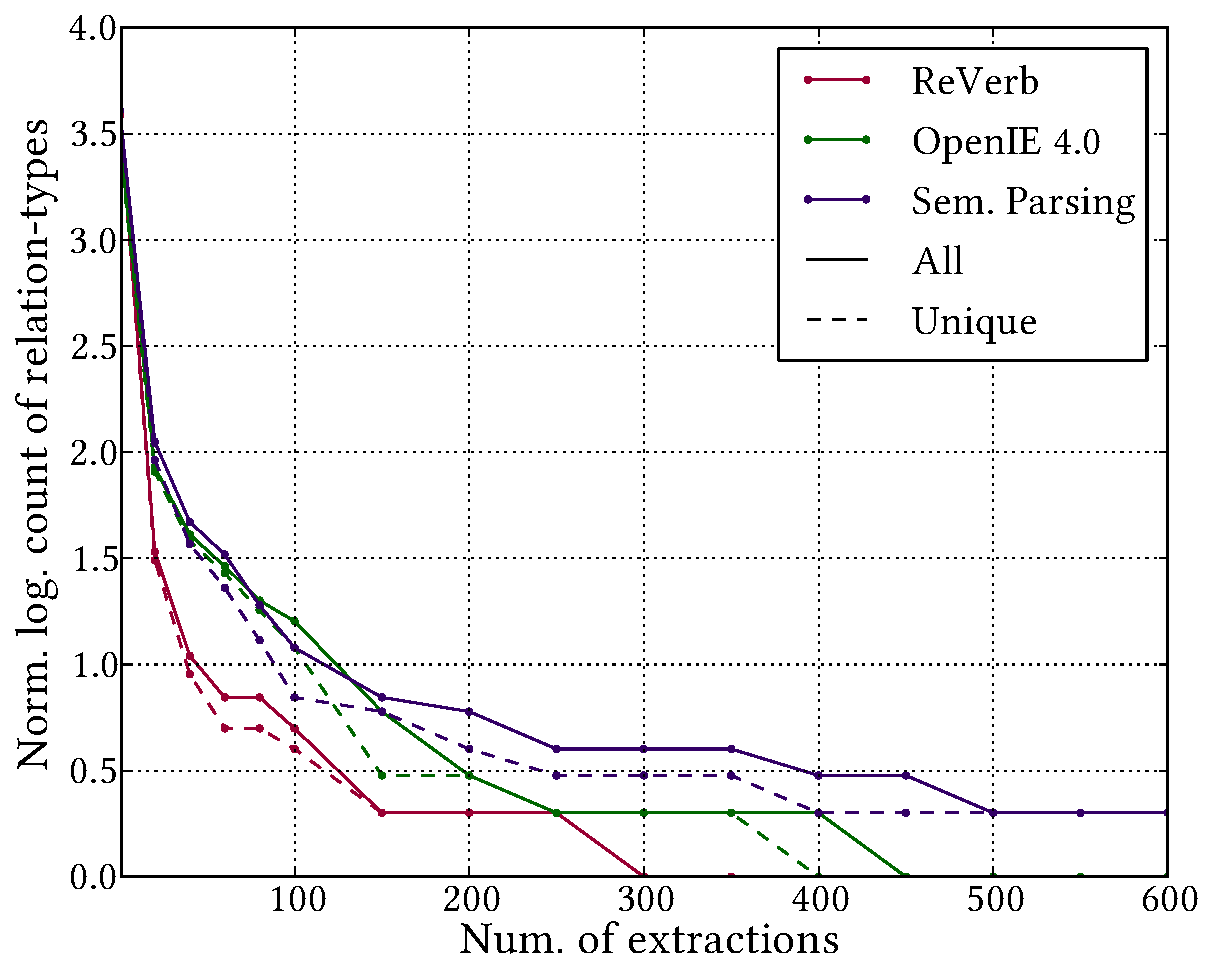
\includegraphics[width=0.45\linewidth]{../data/results/quantitative/carnatic_music/extrations-per-reltype.pdf}
		 \label{fig:quant-reltype-carnatic}
        }% 
        \qquad
        \subfigure[][Hindustani music]{%
		 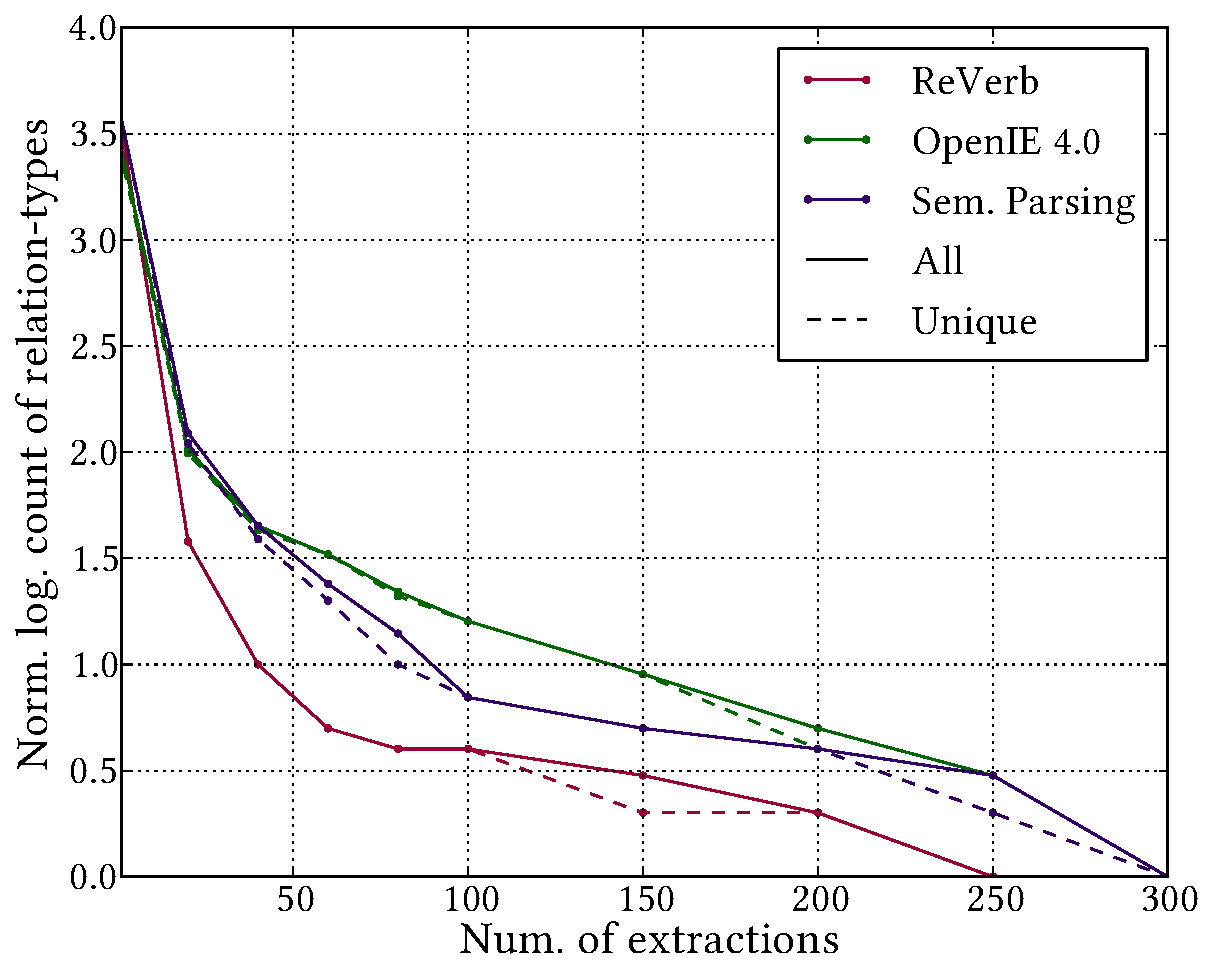
\includegraphics[width=0.45\linewidth]{../data/results/quantitative/hindustani_music/extrations-per-reltype.pdf}
		 \label{fig:quant-reltype-hindustani}
        }%
\end{center}
\caption{Distribution of number of extracted assertions using each of the approaches, per relation type.}
\end{figure}

\begin{figure}
\label{fig:quant-concept}
\begin{center}
        \subfigure[][Carnatic music]{%
		 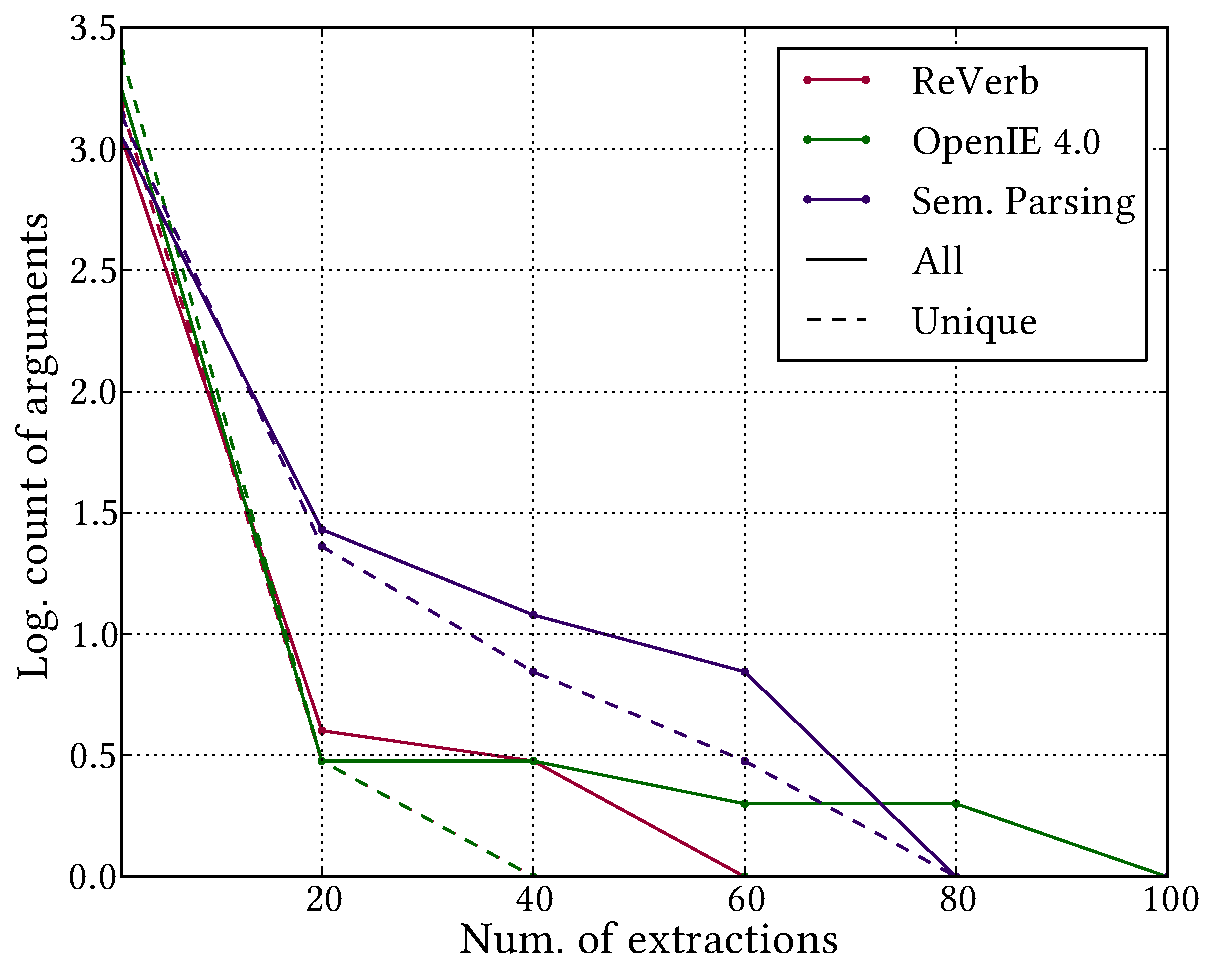
\includegraphics[width=0.45\linewidth]{../data/results/quantitative/carnatic_music/extrations-per-class.pdf}
		 \label{fig:quant-concept-carnatic}
        }% 
        \qquad
        \subfigure[][Hindustani music]{%
		 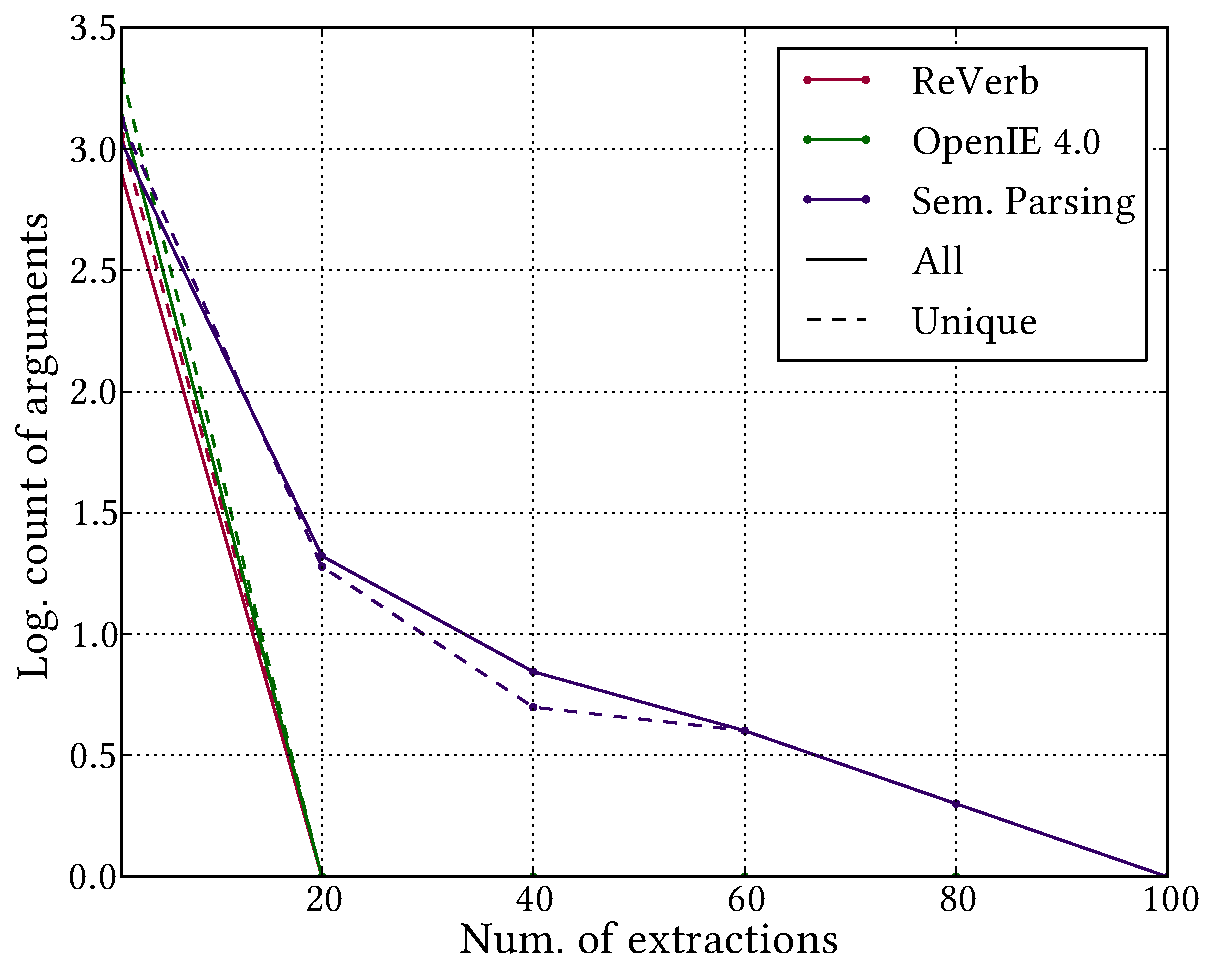
\includegraphics[width=0.45\linewidth]{../data/results/quantitative/hindustani_music/extrations-per-class.pdf}
		 \label{fig:quant-concept-hindustani}
        }%
\end{center}
\caption{Distribution of number of extracted assertions using each of the approaches, per concept.}
\end{figure}

\subsection{Qualitative assessment}
\subsubsection{Object identification.}
\begin{figure}
\label{fig:qual-object-rulebased}
\begin{center}
        \subfigure[][Carnatic music]{%
		 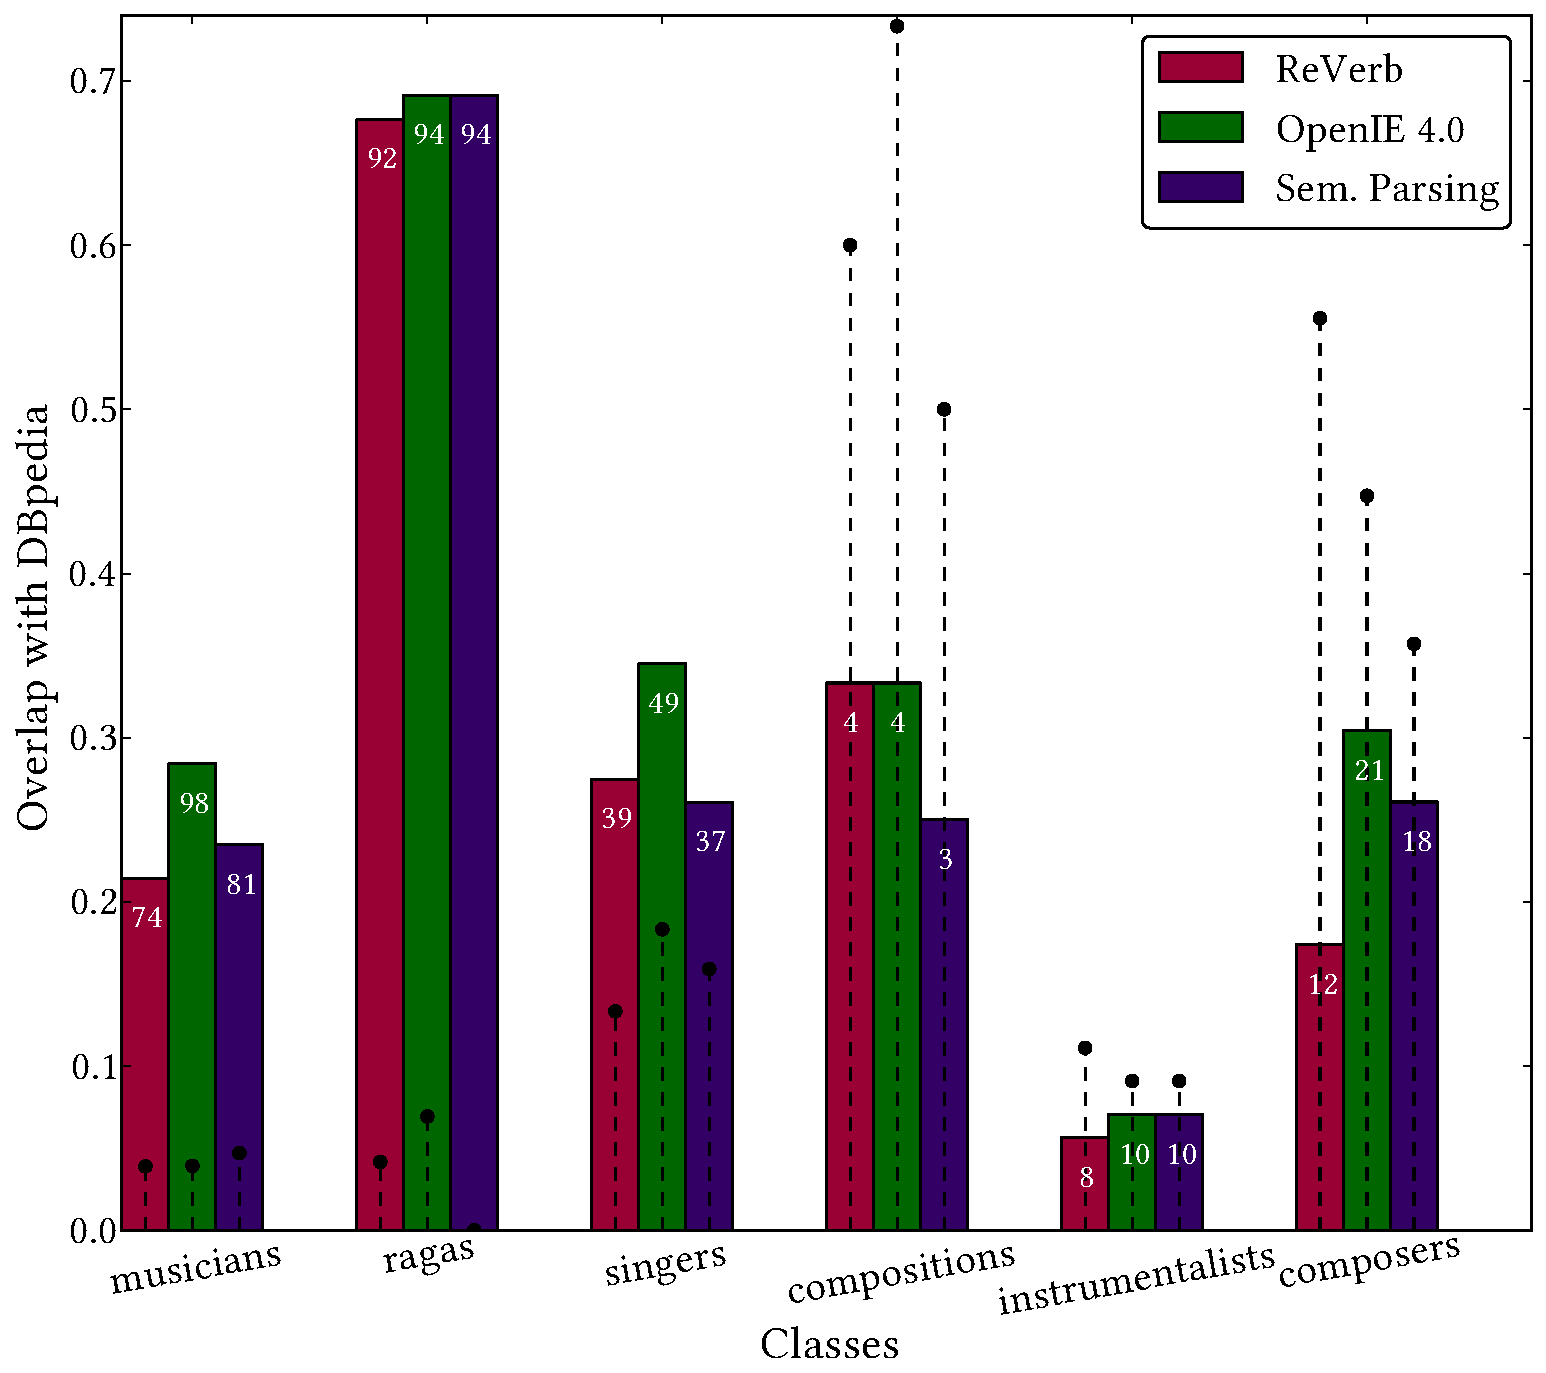
\includegraphics[width=0.45\linewidth]{../data/results/qualitative/object-identification/rule-based/carnatic_music/class-agreement-with-wikipedia.pdf}
		 \label{fig:qual-object-rulebased-carnatic}
        }% 
        \qquad
        \subfigure[][Hindustani music]{%
		 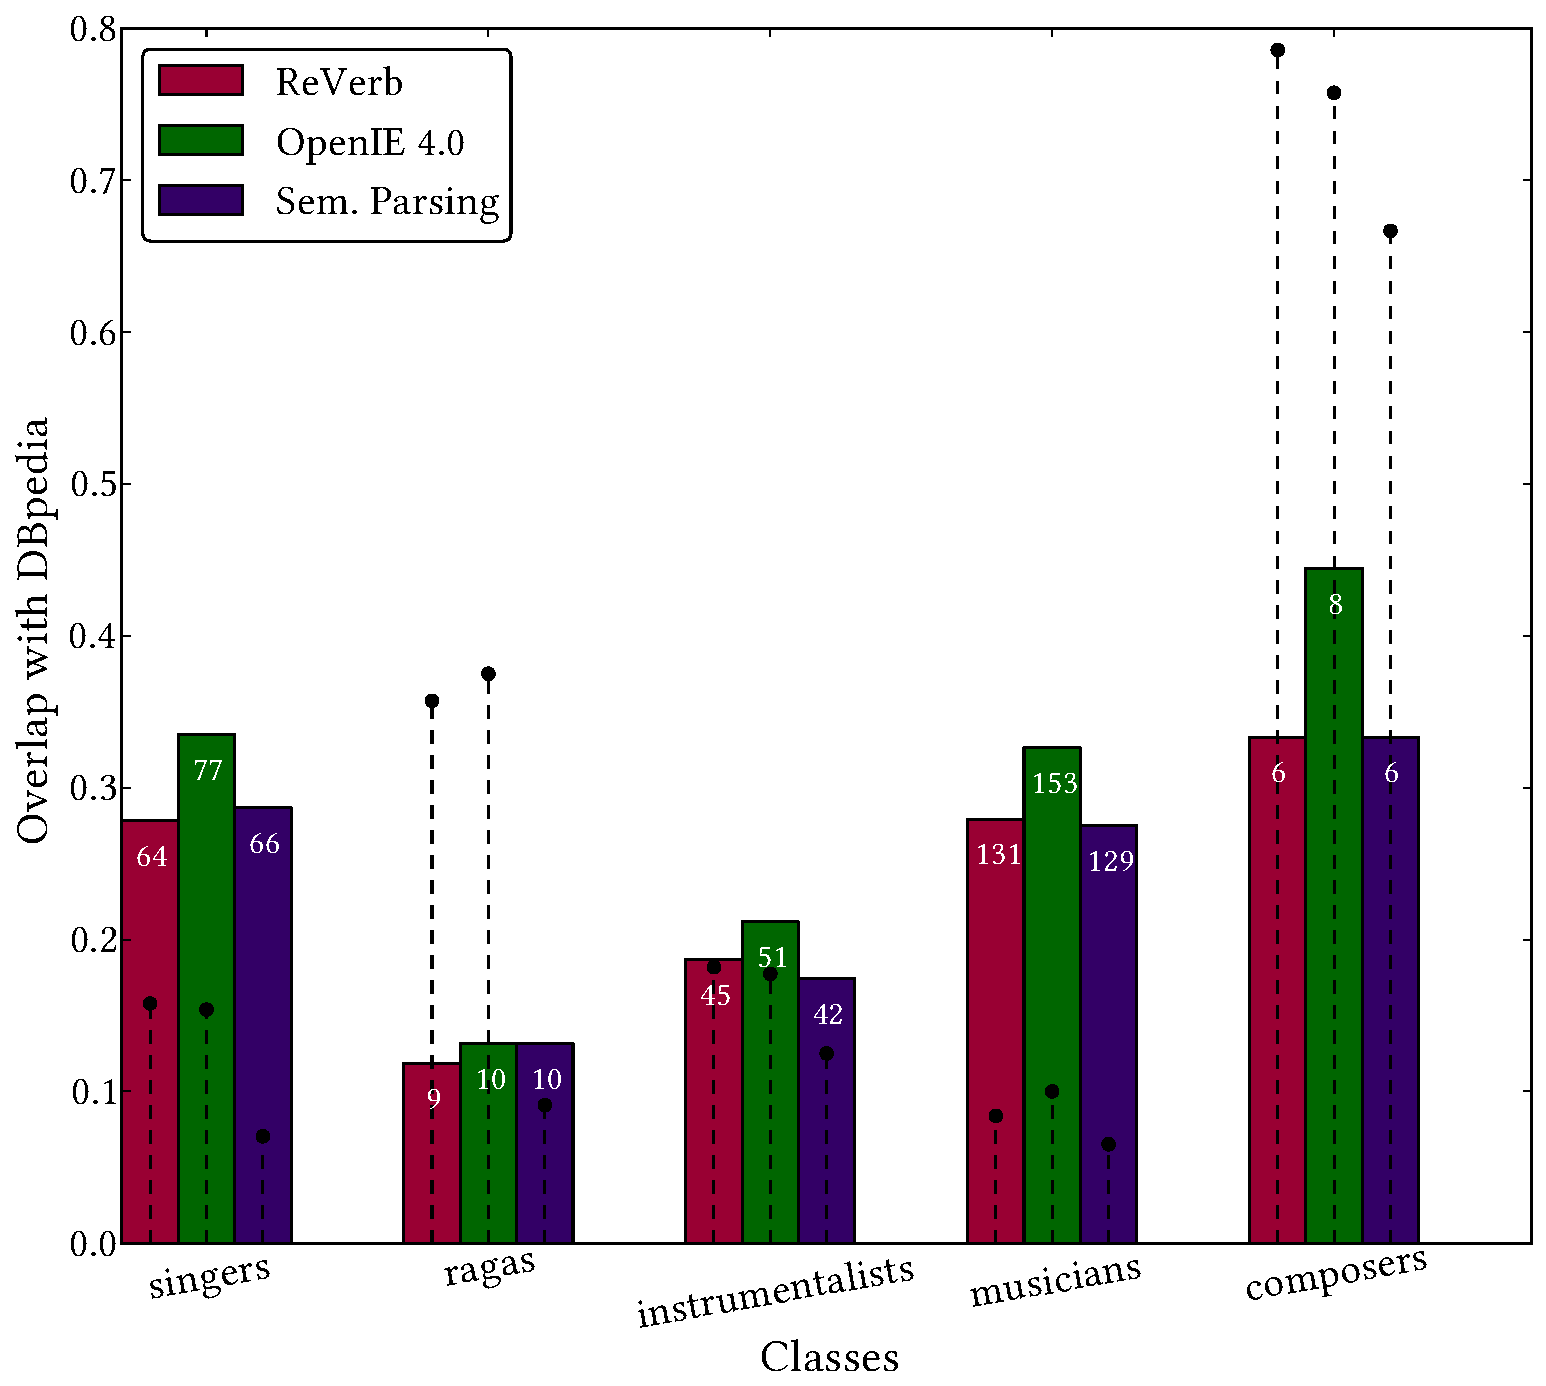
\includegraphics[width=0.45\linewidth]{../data/results/qualitative/object-identification/rule-based/hindustani_music/class-agreement-with-wikipedia.pdf}
		 \label{fig:qual-object-rulebased-hindustani}
        }%
\end{center}
\caption{Results for rule-based semantic category assignment to objects identified in the domain.}
\end{figure}

\begin{figure}
\label{fig:qual-object-rulebased-inter}
\begin{center}
        \subfigure[][Carnatic music]{%
		 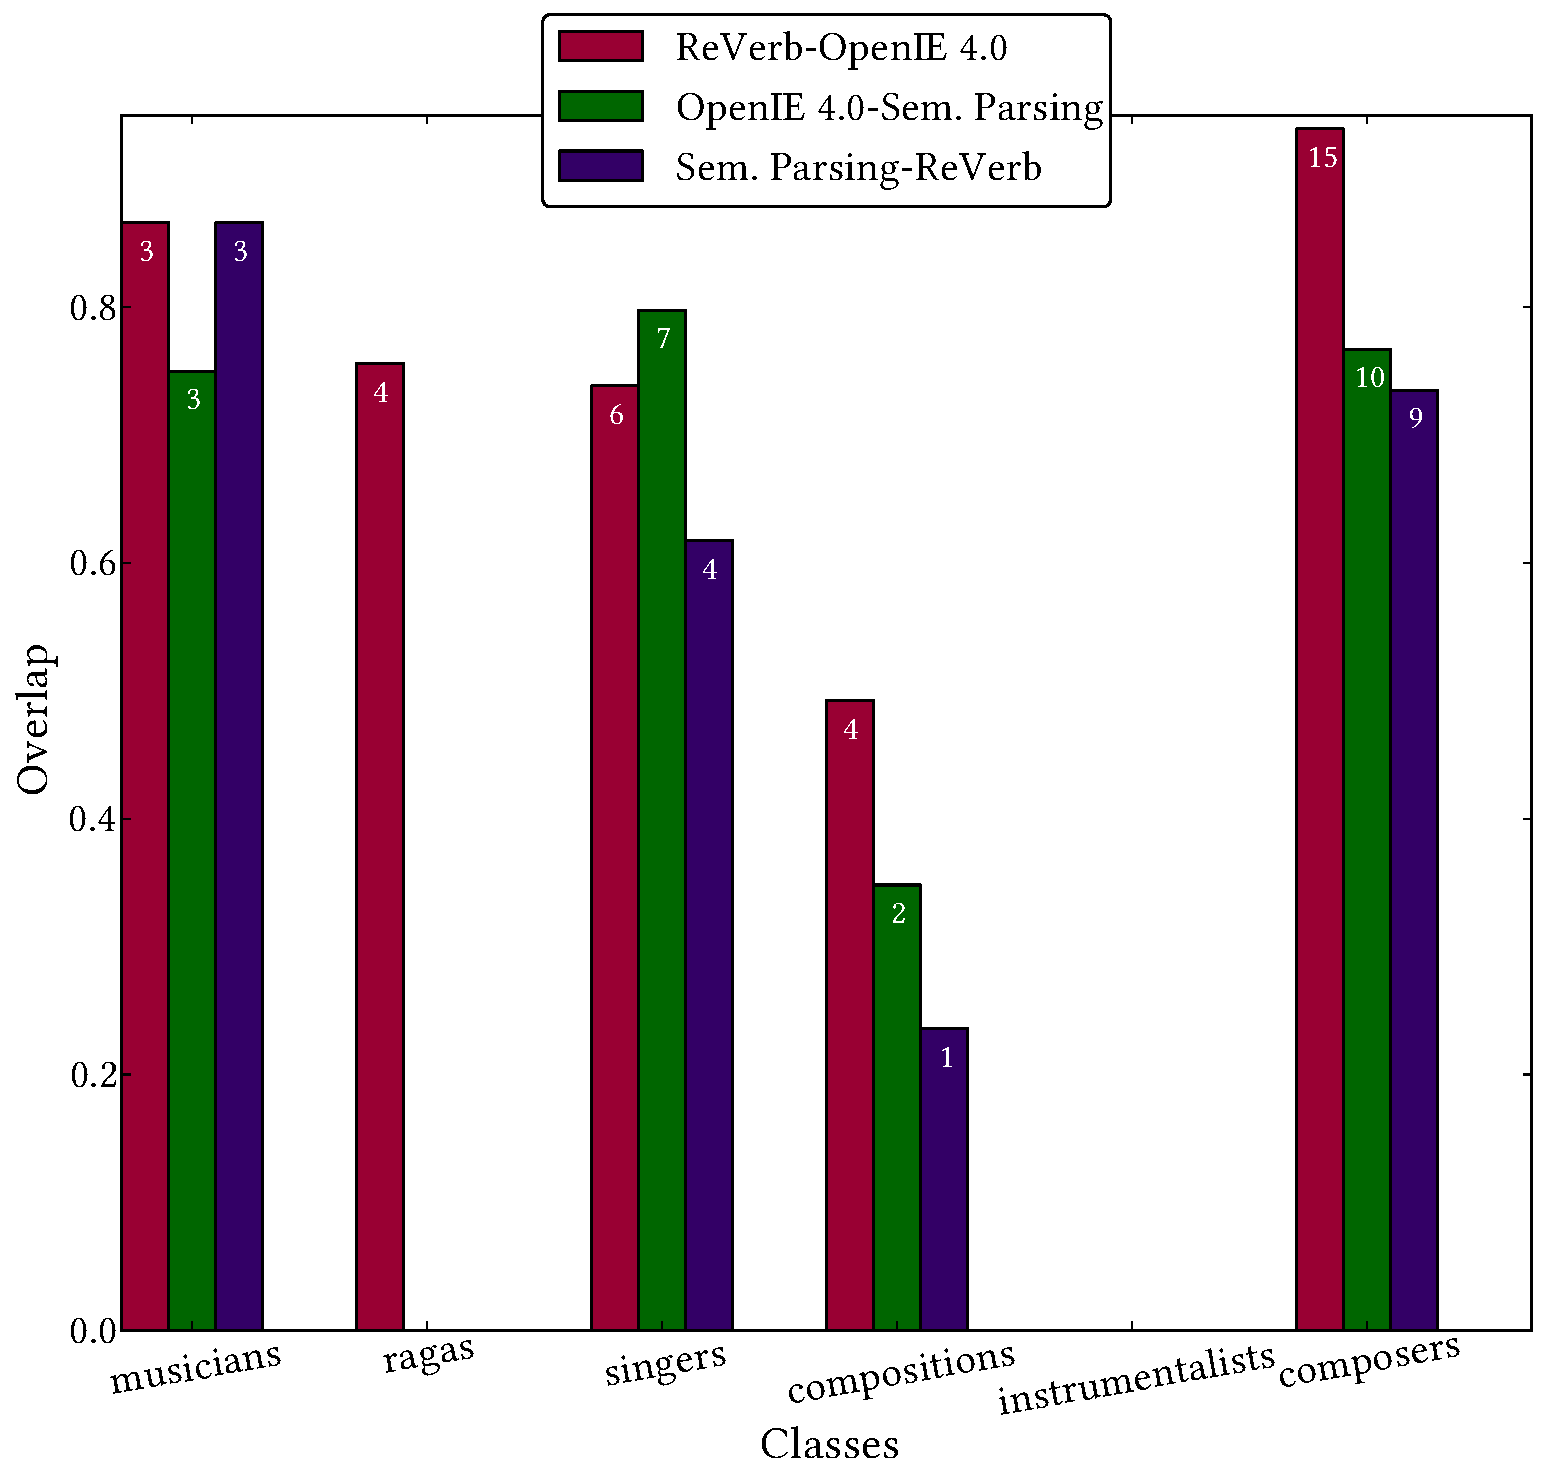
\includegraphics[width=0.45\linewidth]{../data/results/qualitative/object-identification/rule-based/carnatic_music/class-agreement-inter-method.pdf}
		 \label{fig:qual-object-rulebased-inter-carnatic}
        }% 
        \qquad
        \subfigure[][Hindustani music]{%
		 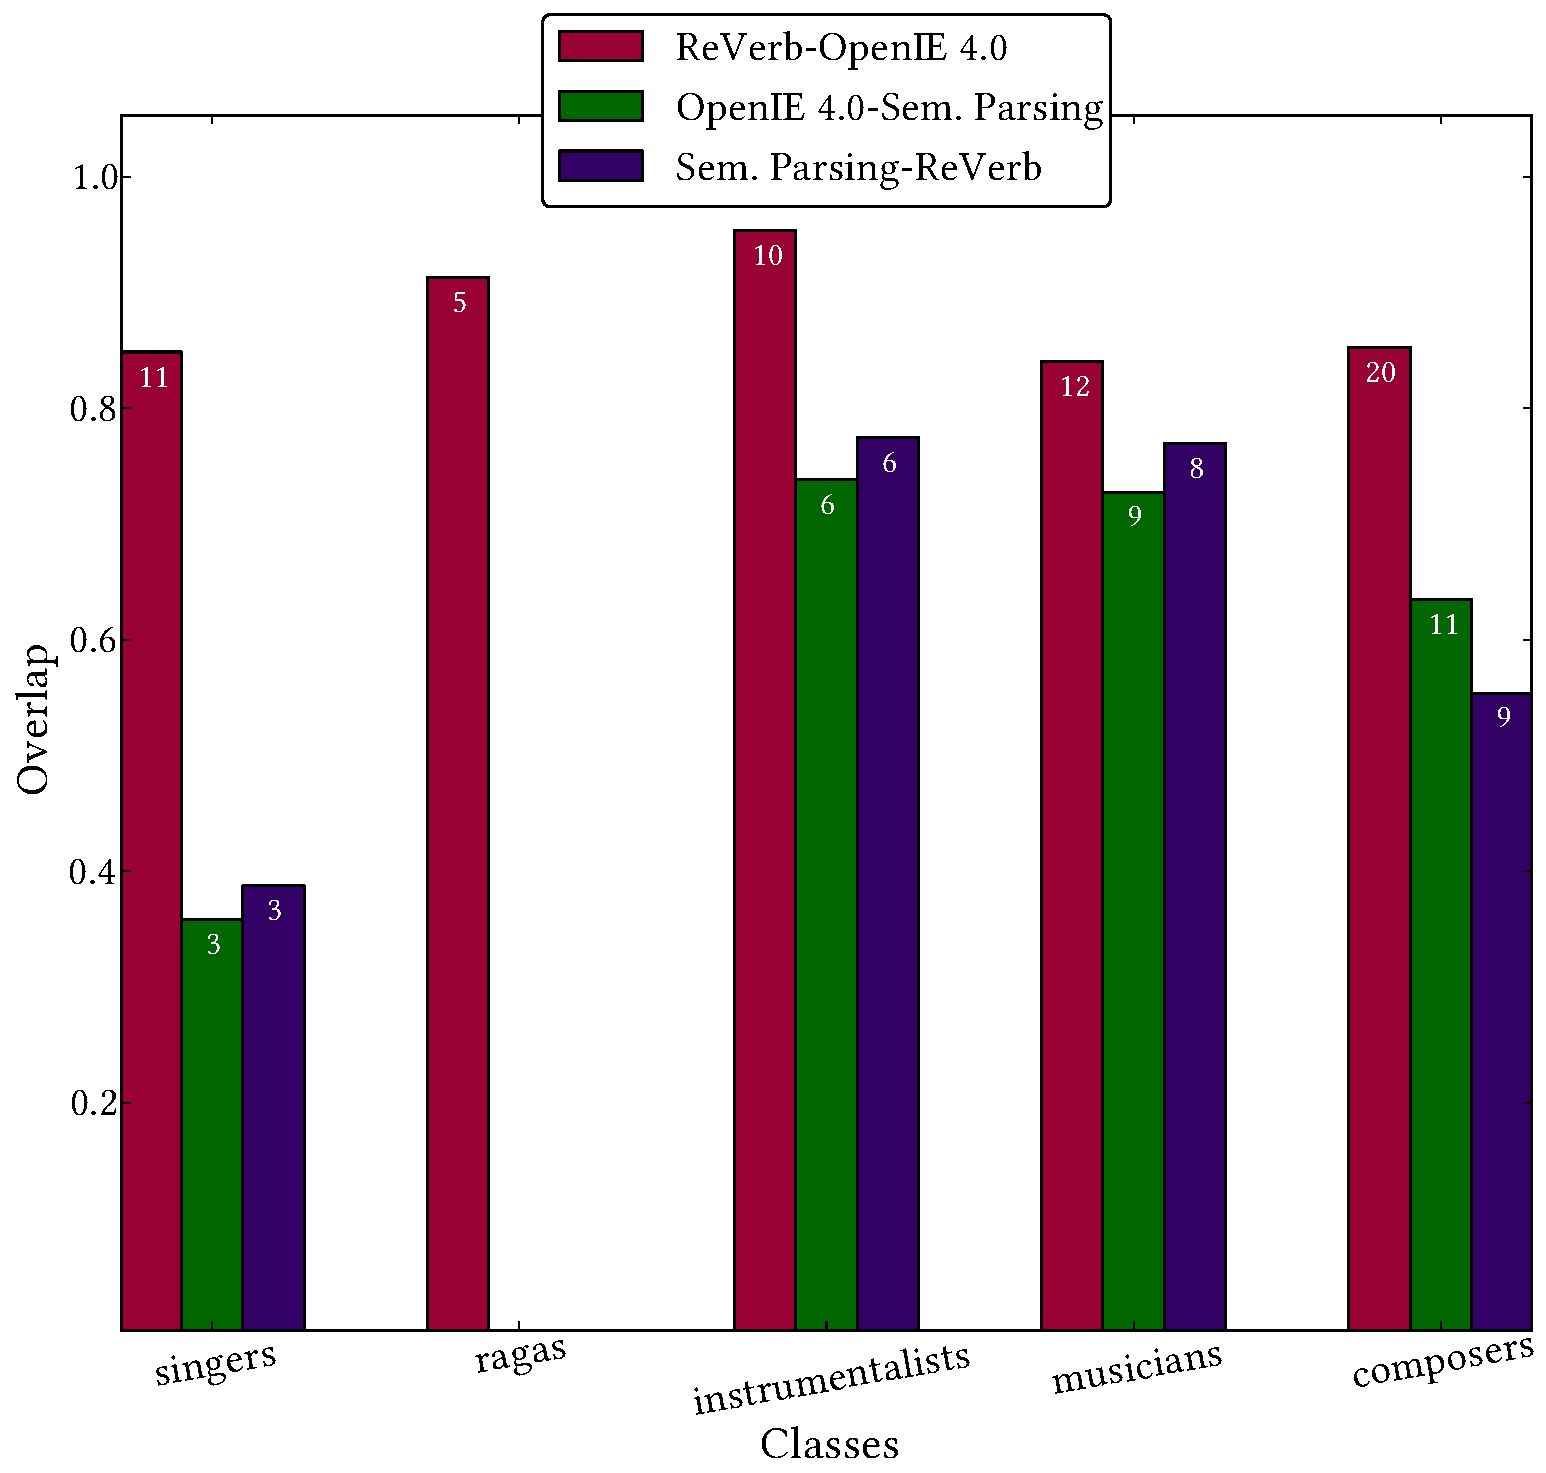
\includegraphics[width=0.45\linewidth]{../data/results/qualitative/object-identification/rule-based/hindustani_music/class-agreement-inter-method.pdf}
		 \label{fig:qual-object-rulebased-inter-hindustani}
        }%
\end{center}
\caption{Inter-approach agreement for semantic category assignment of the objects that correspond to false positives by our reference data.}
\end{figure}

\begin{figure}
\label{fig:qual-object-bootstrapping-carnatic}
\begin{center}
        \subfigure[][Musicians]{%
		 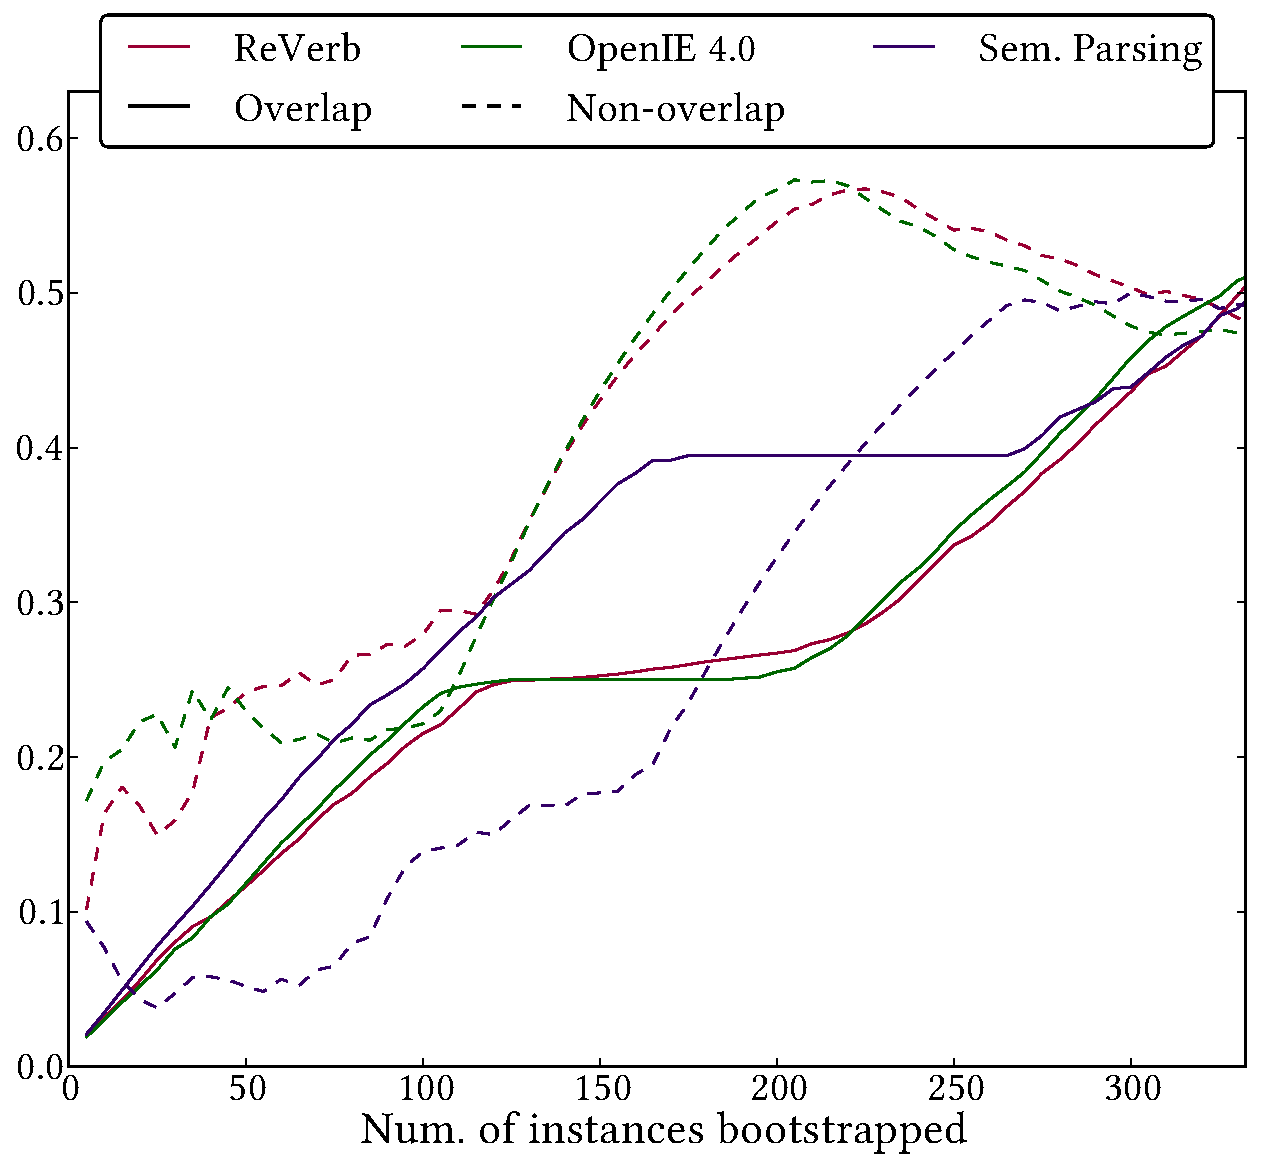
\includegraphics[width=0.45\linewidth]{../data/results/qualitative/object-identification/bootstrapping/carnatic_music/carnatic_musicians.pdf}
		 \label{fig:qual-object-bootstrapping-carnatic-musicians}
        }% 
        \qquad
        \subfigure[][Composers]{%
		 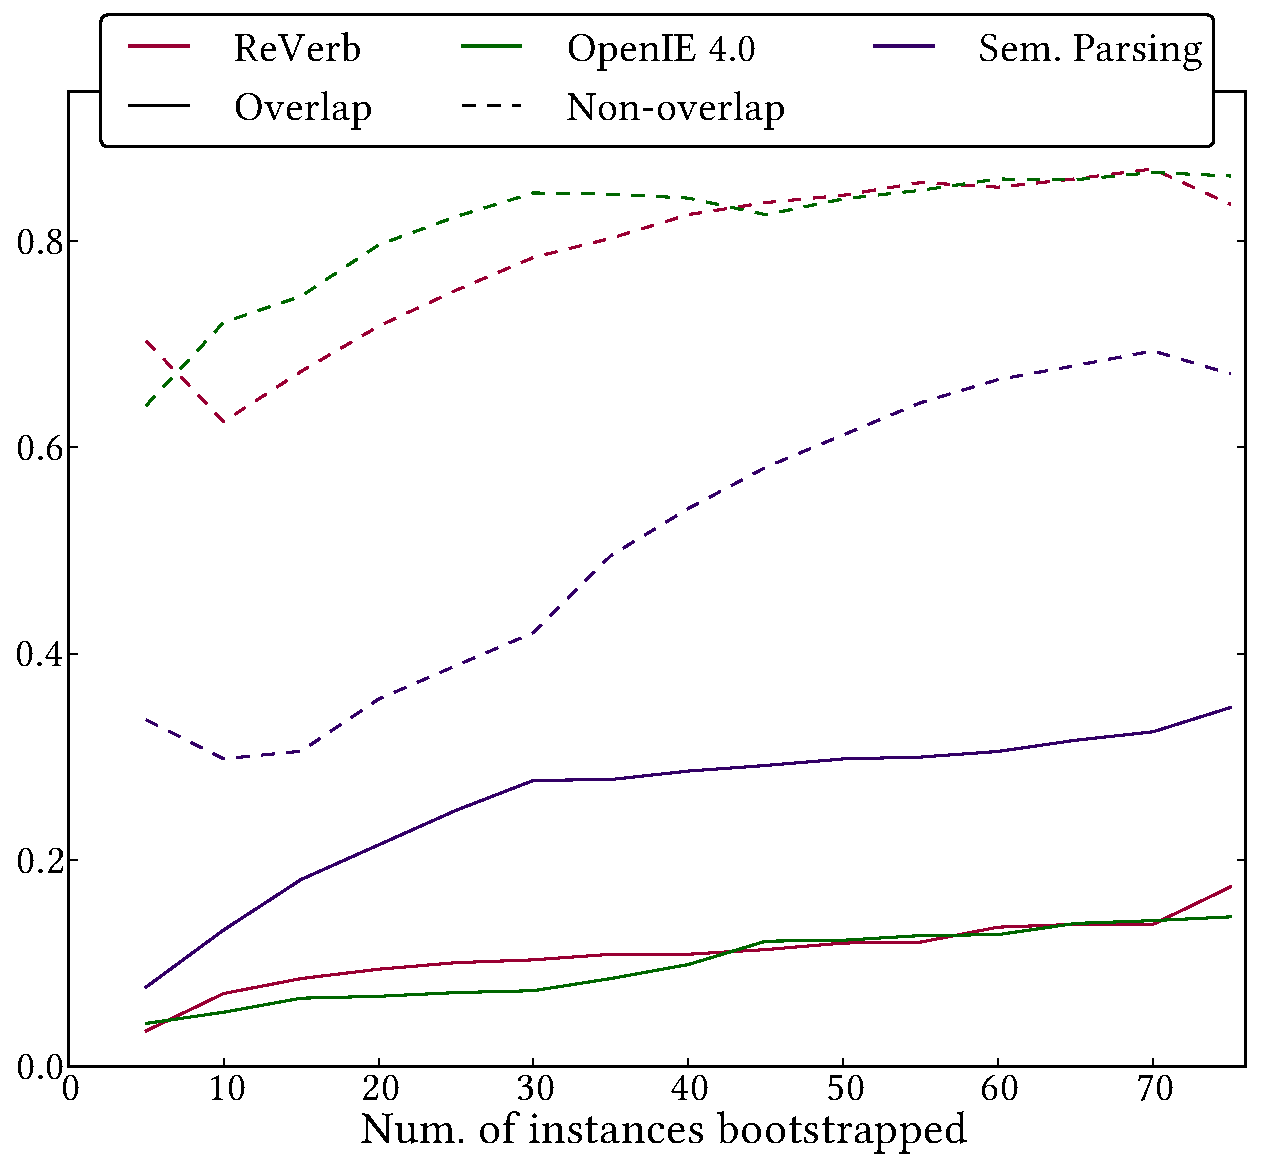
\includegraphics[width=0.45\linewidth]{../data/results/qualitative/object-identification/bootstrapping/carnatic_music/carnatic_composers.pdf}
		 \label{fig:qual-object-bootstrapping-carnatic-composers}
        }%
        \\
        \subfigure[][Instrumentalists]{%
		 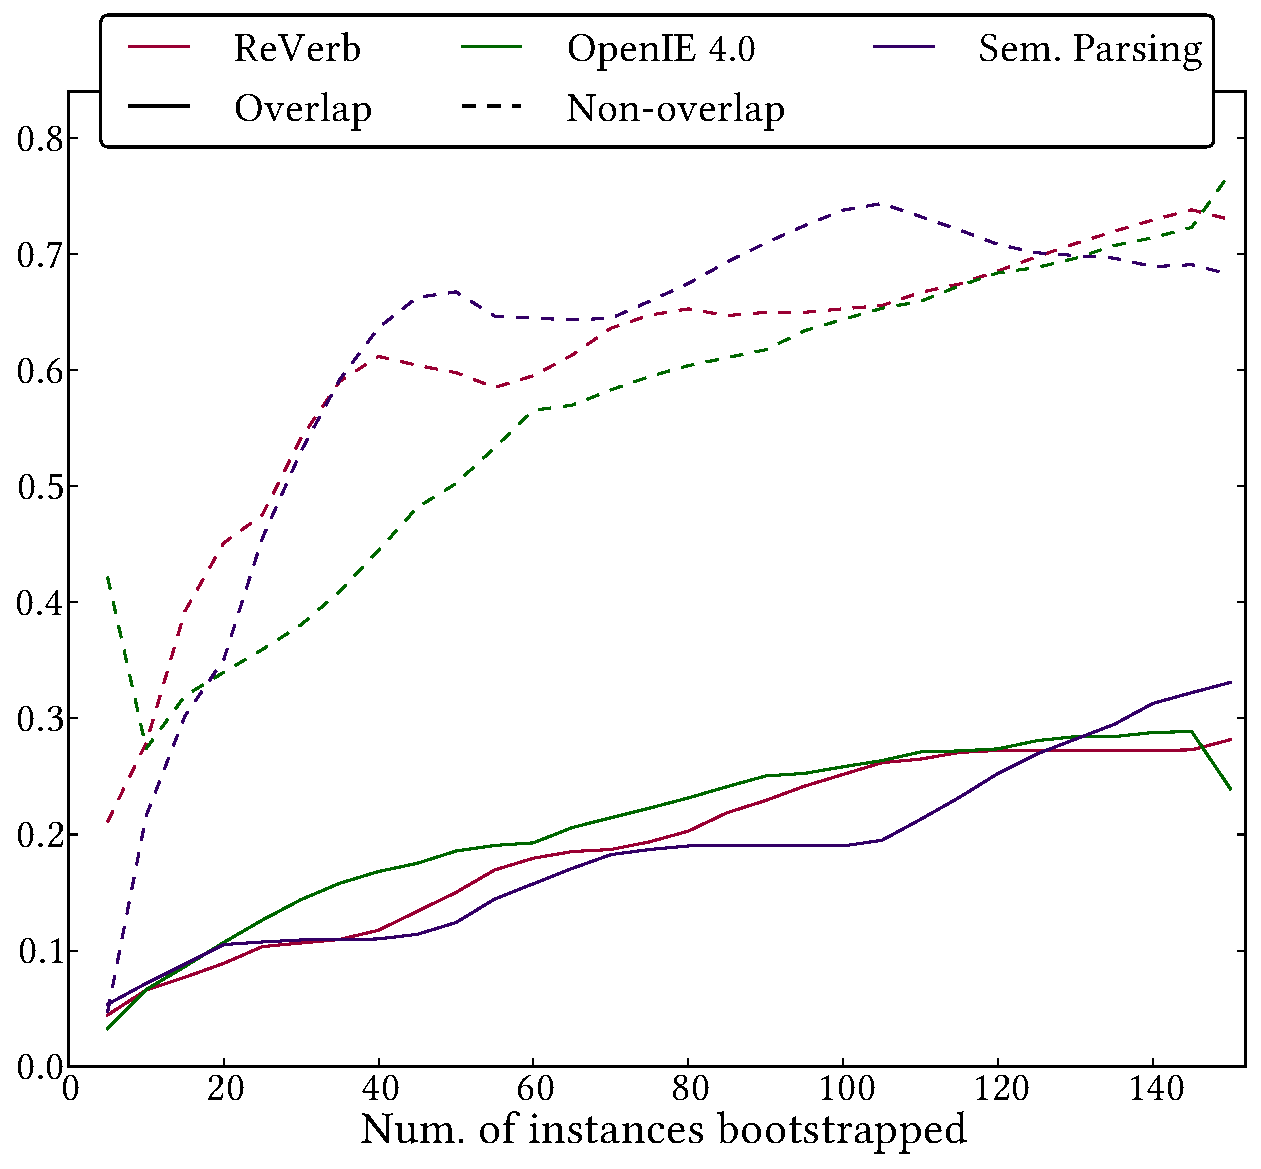
\includegraphics[width=0.45\linewidth]{../data/results/qualitative/object-identification/bootstrapping/carnatic_music/carnatic_instrumentalists.pdf}
		 \label{fig:qual-object-bootstrapping-carnatic-instrumentalists}
        }% 
        \qquad
        \subfigure[][Singers]{%
		 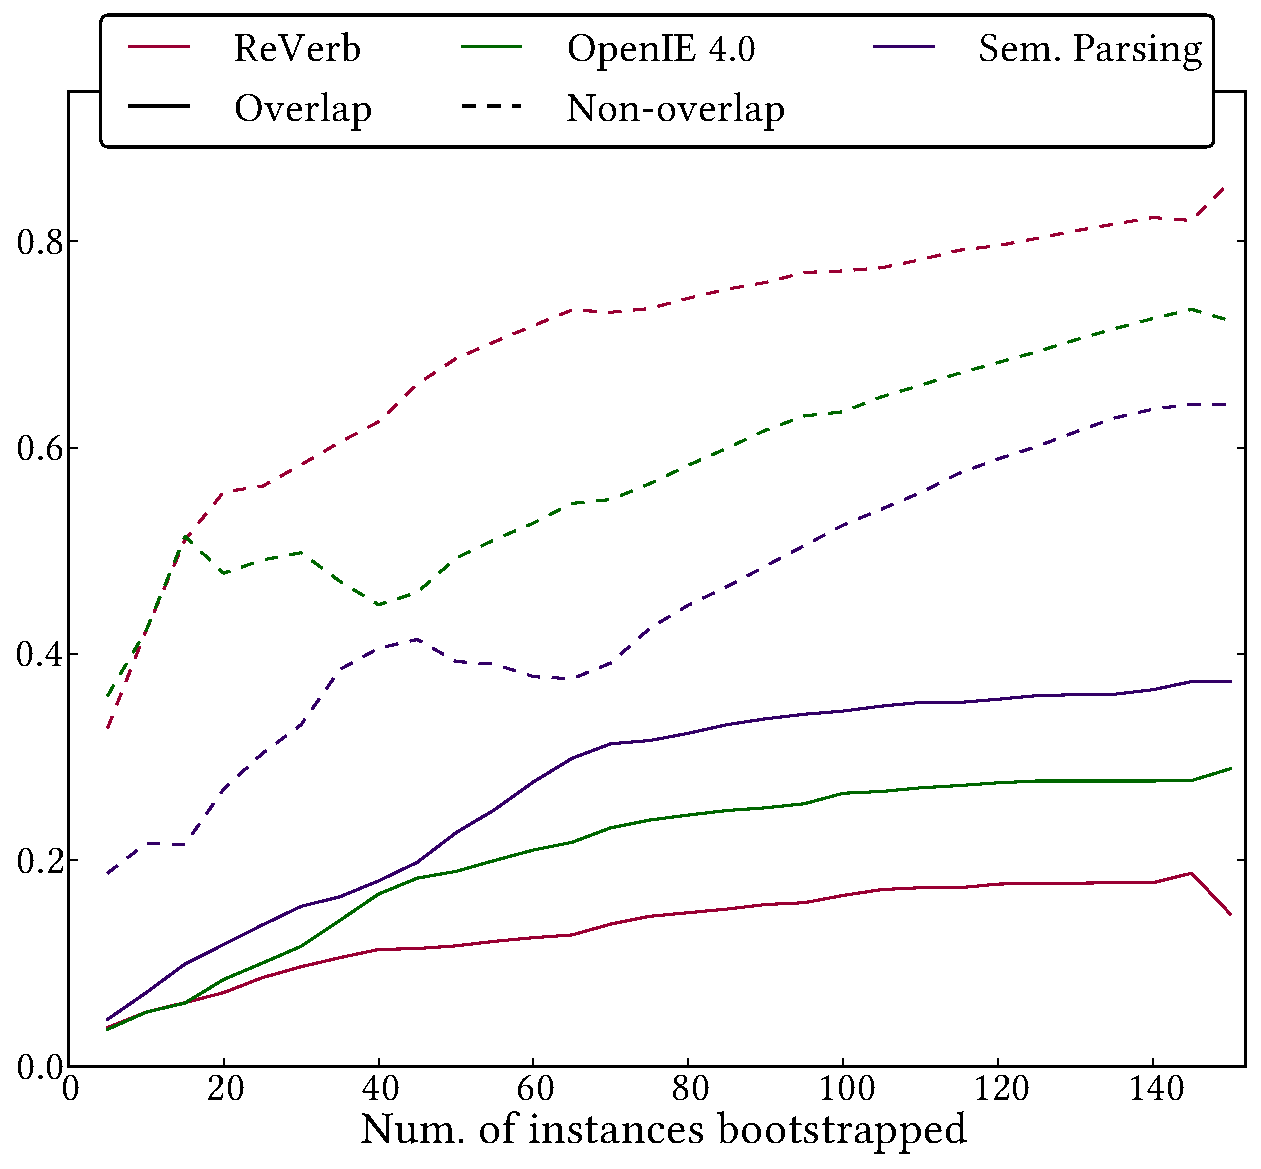
\includegraphics[width=0.45\linewidth]{../data/results/qualitative/object-identification/bootstrapping/carnatic_music/carnatic_singers.pdf}
		 \label{fig:qual-object-bootstrapping-carnatic-singers}
        }%
        \\
        \subfigure[][Ragas]{%
		 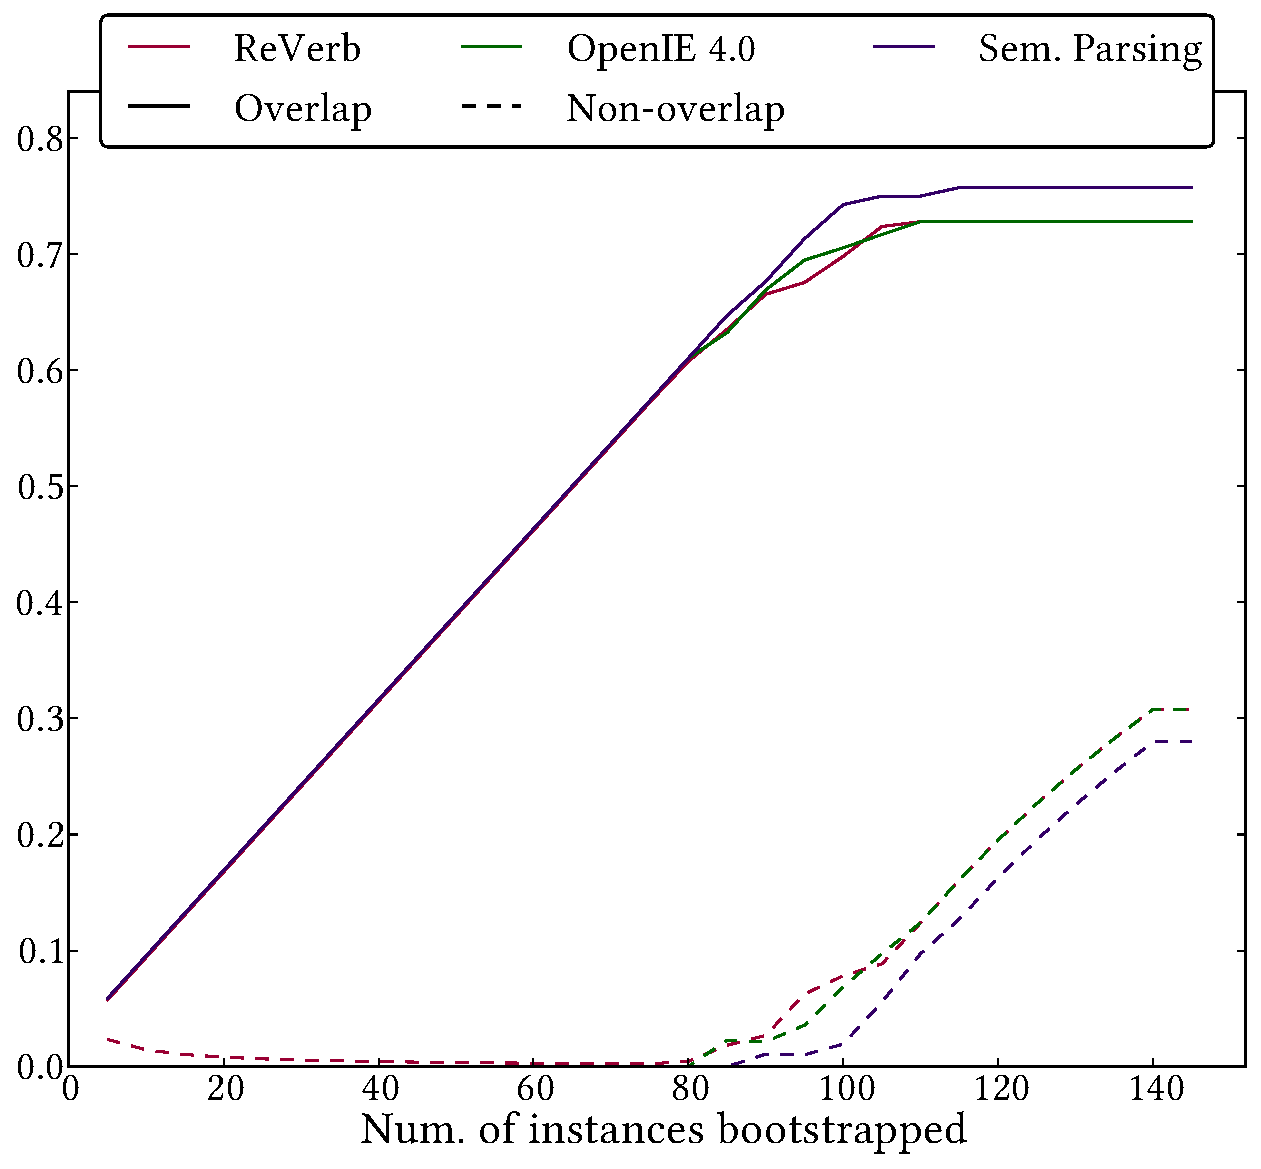
\includegraphics[width=0.45\linewidth]{../data/results/qualitative/object-identification/bootstrapping/carnatic_music/carnatic_ragas.pdf}
		 \label{fig:qual-object-bootstrapping-carnatic-ragas}
        }% 
        \qquad
        \subfigure[][Compositions]{%
		 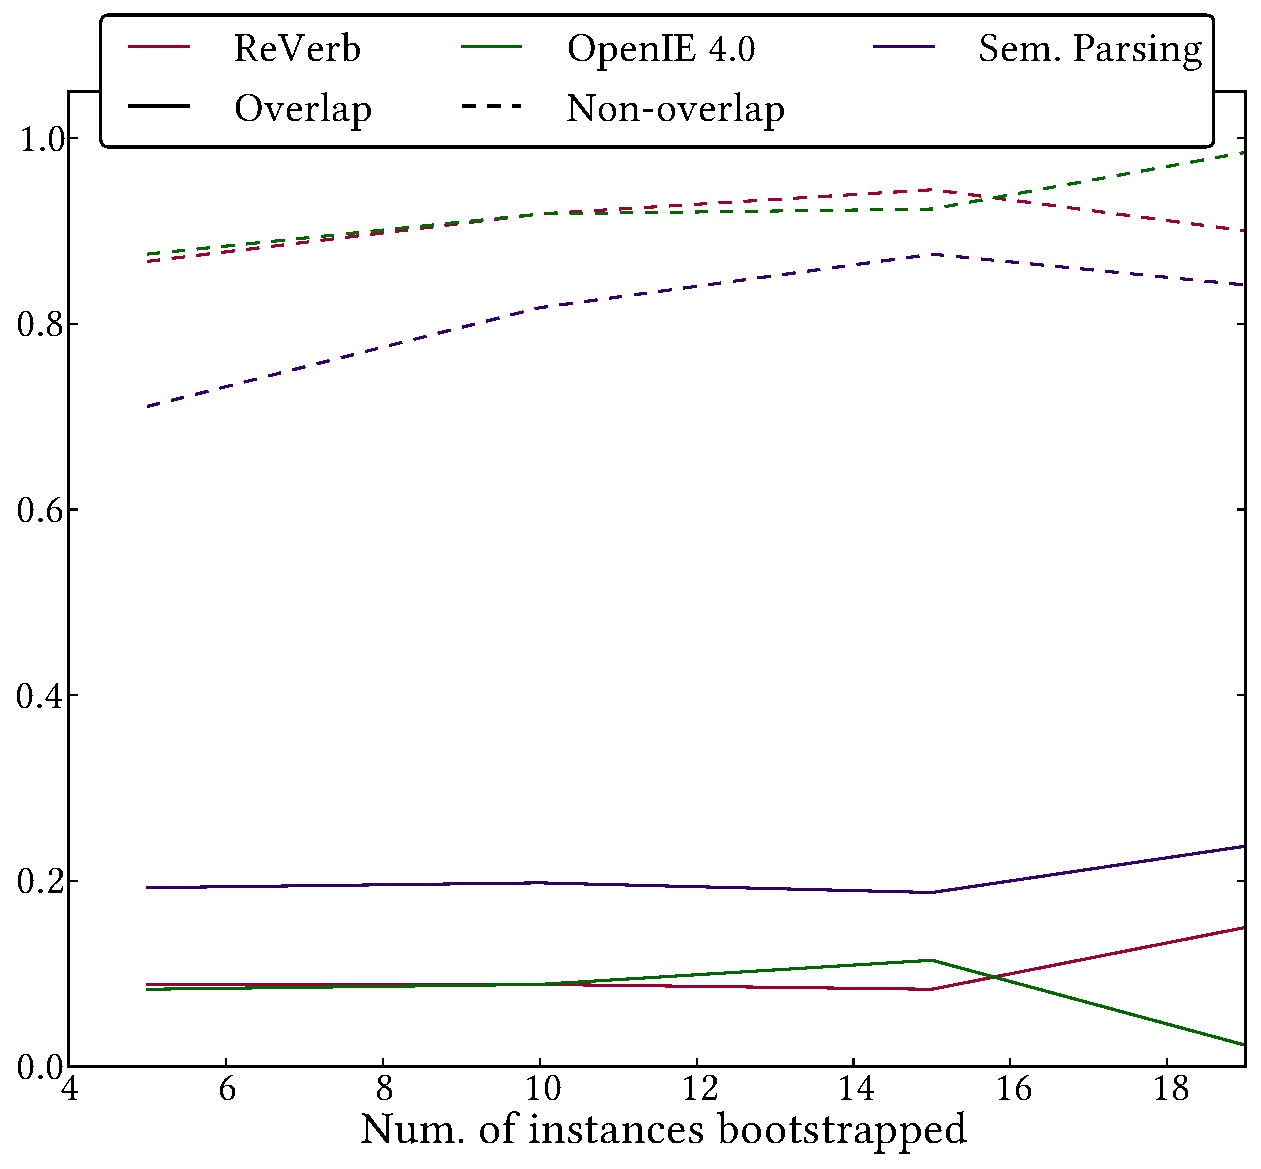
\includegraphics[width=0.45\linewidth]{../data/results/qualitative/object-identification/bootstrapping/carnatic_music/carnatic_compositions.pdf}
		 \label{fig:qual-object-bootstrapping-carnatic-compositions}
        }%
\end{center}
\caption{Carnatic Results.}
\end{figure}

\begin{figure}
\label{fig:qual-object-bootstrapping-hindustani}
\begin{center}
        \subfigure[][Musicians]{%
		 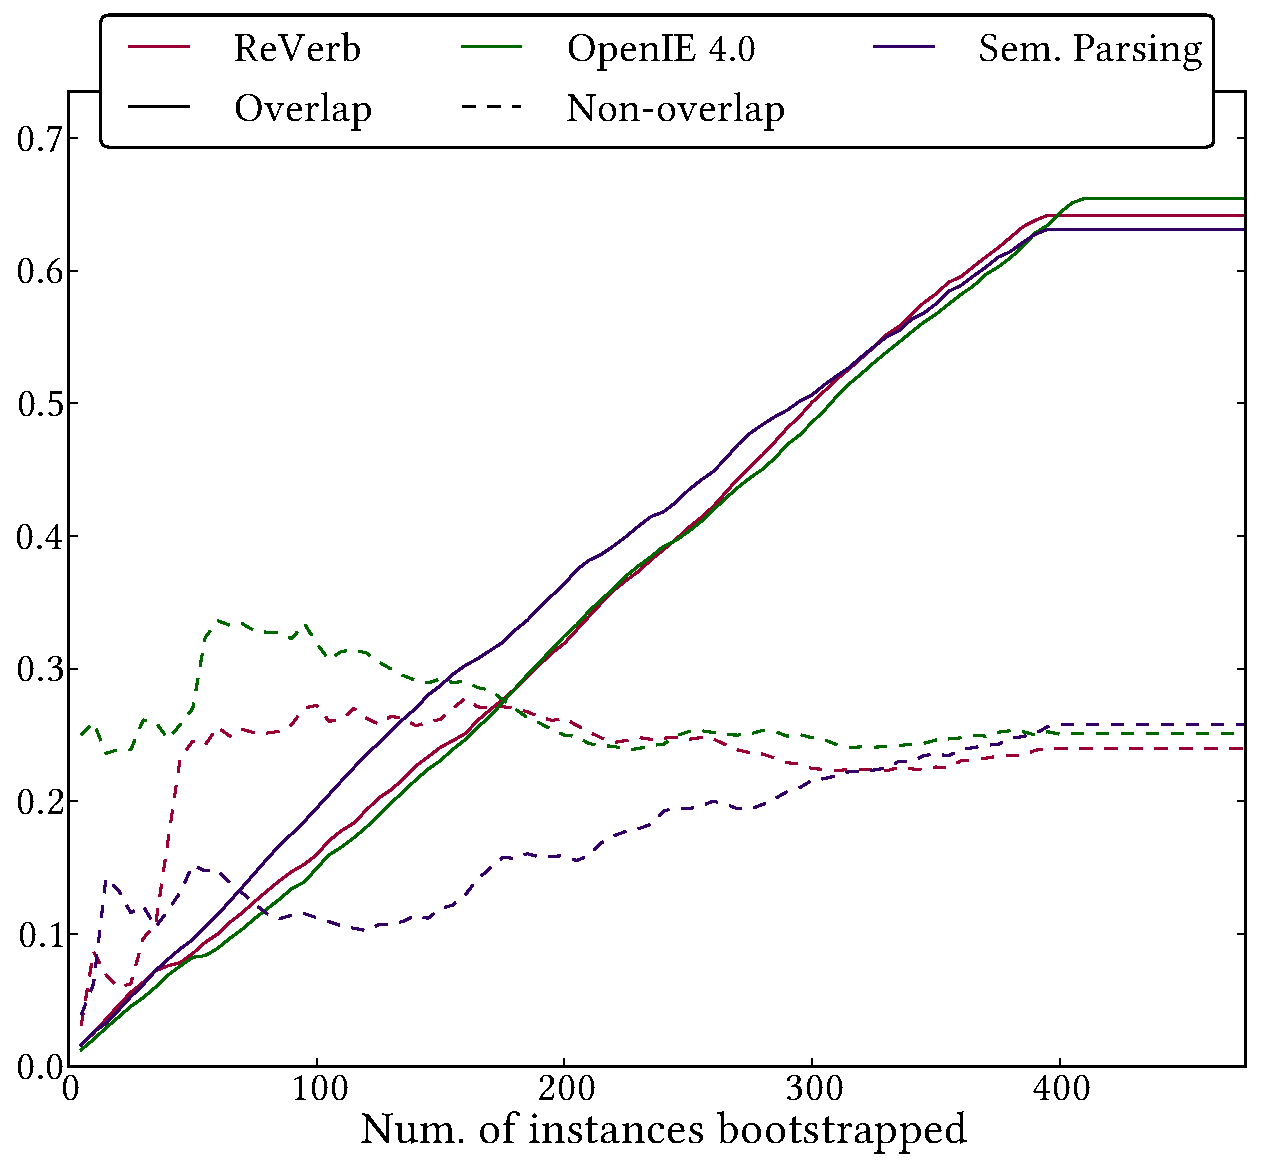
\includegraphics[width=0.45\linewidth]{../data/results/qualitative/object-identification/bootstrapping/hindustani_music/hindustani_musicians.pdf}
		 \label{fig:qual-object-bootstrapping-hindustani-musicians}
        }% 
        \qquad
        \subfigure[][Composers]{%
		 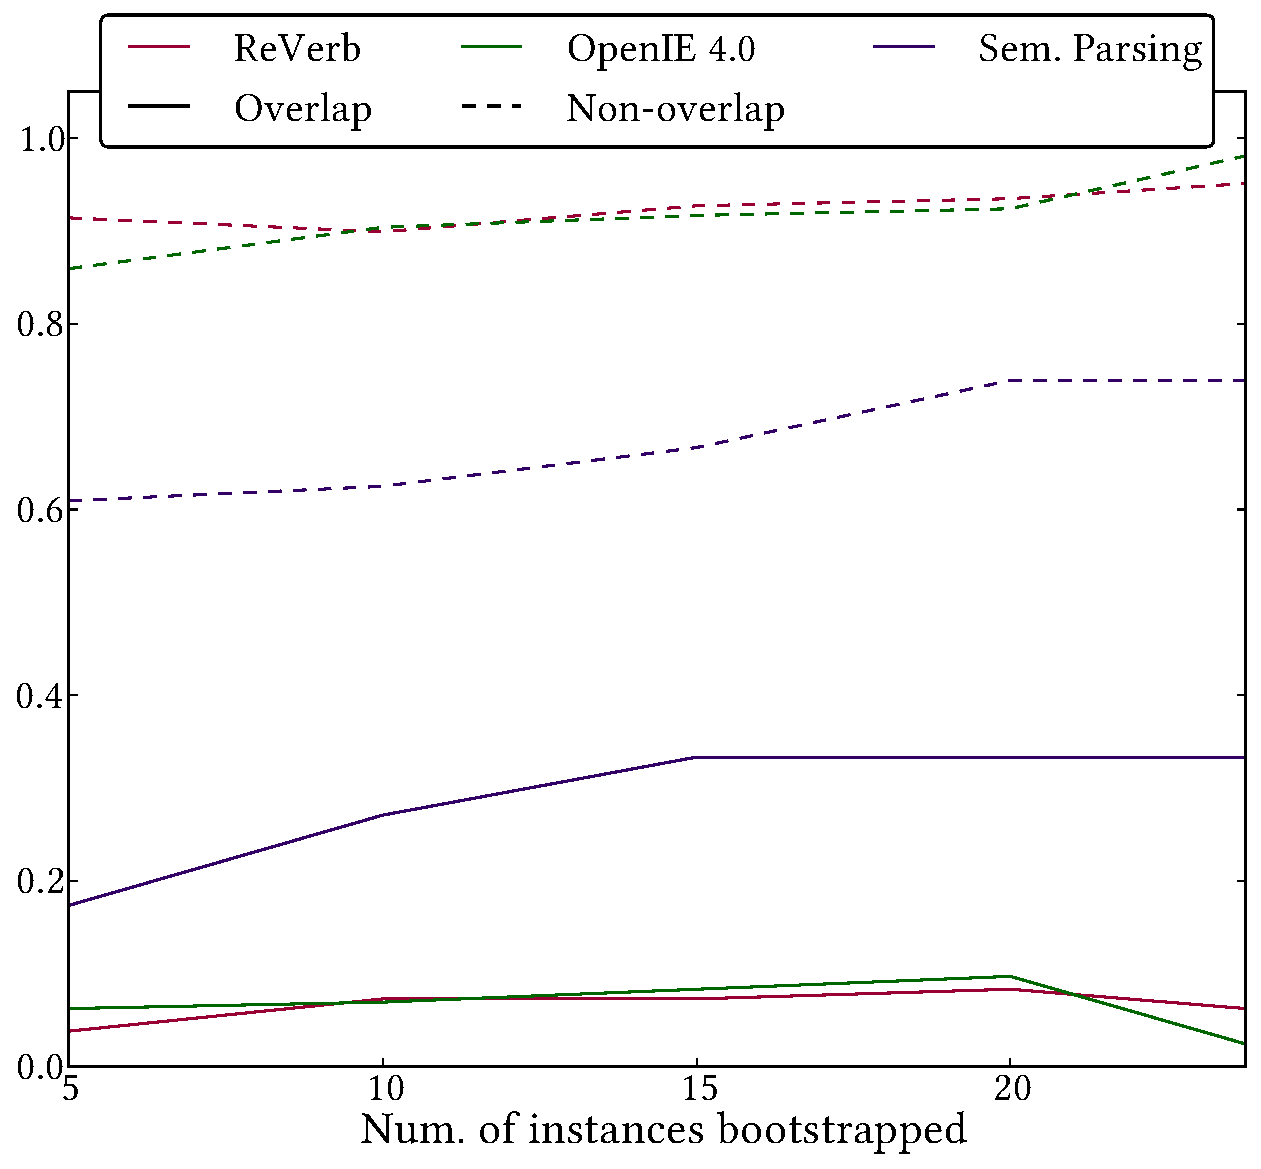
\includegraphics[width=0.45\linewidth]{../data/results/qualitative/object-identification/bootstrapping/hindustani_music/hindustani_composers.pdf}
		 \label{fig:qual-object-bootstrapping-hindustani-composers}
        }%
        \\
        \subfigure[][Instrumentalists]{%
		 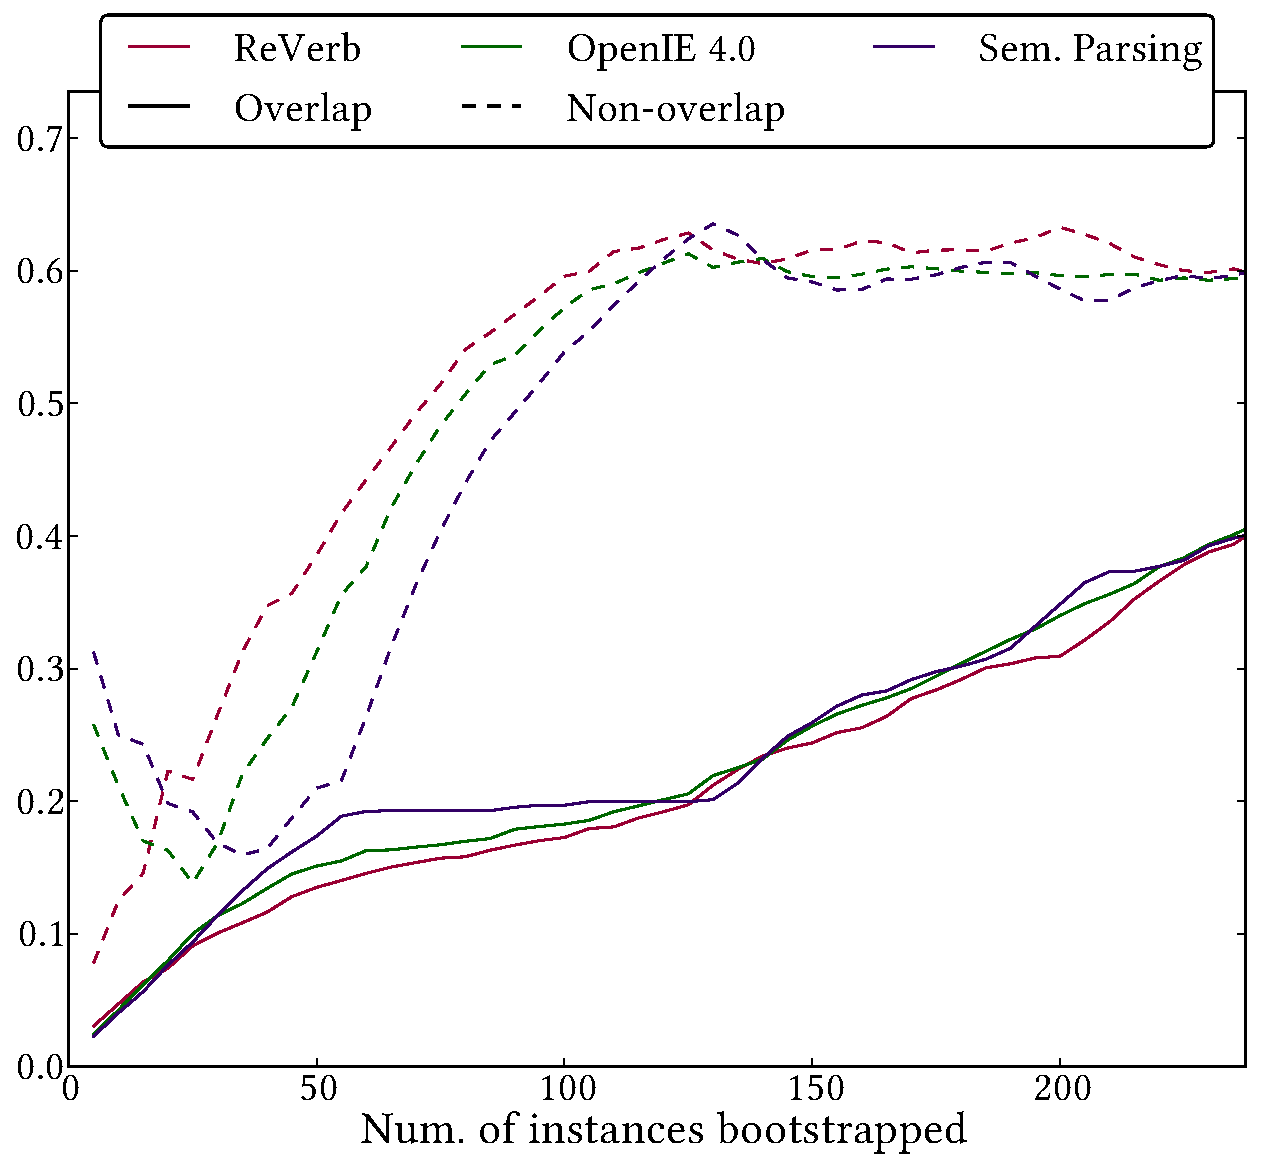
\includegraphics[width=0.45\linewidth]{../data/results/qualitative/object-identification/bootstrapping/hindustani_music/hindustani_instrumentalists.pdf}
		 \label{fig:qual-object-bootstrapping-hindustani-instrumentalists}
        }% 
        \qquad
        \subfigure[][Singers]{%
		 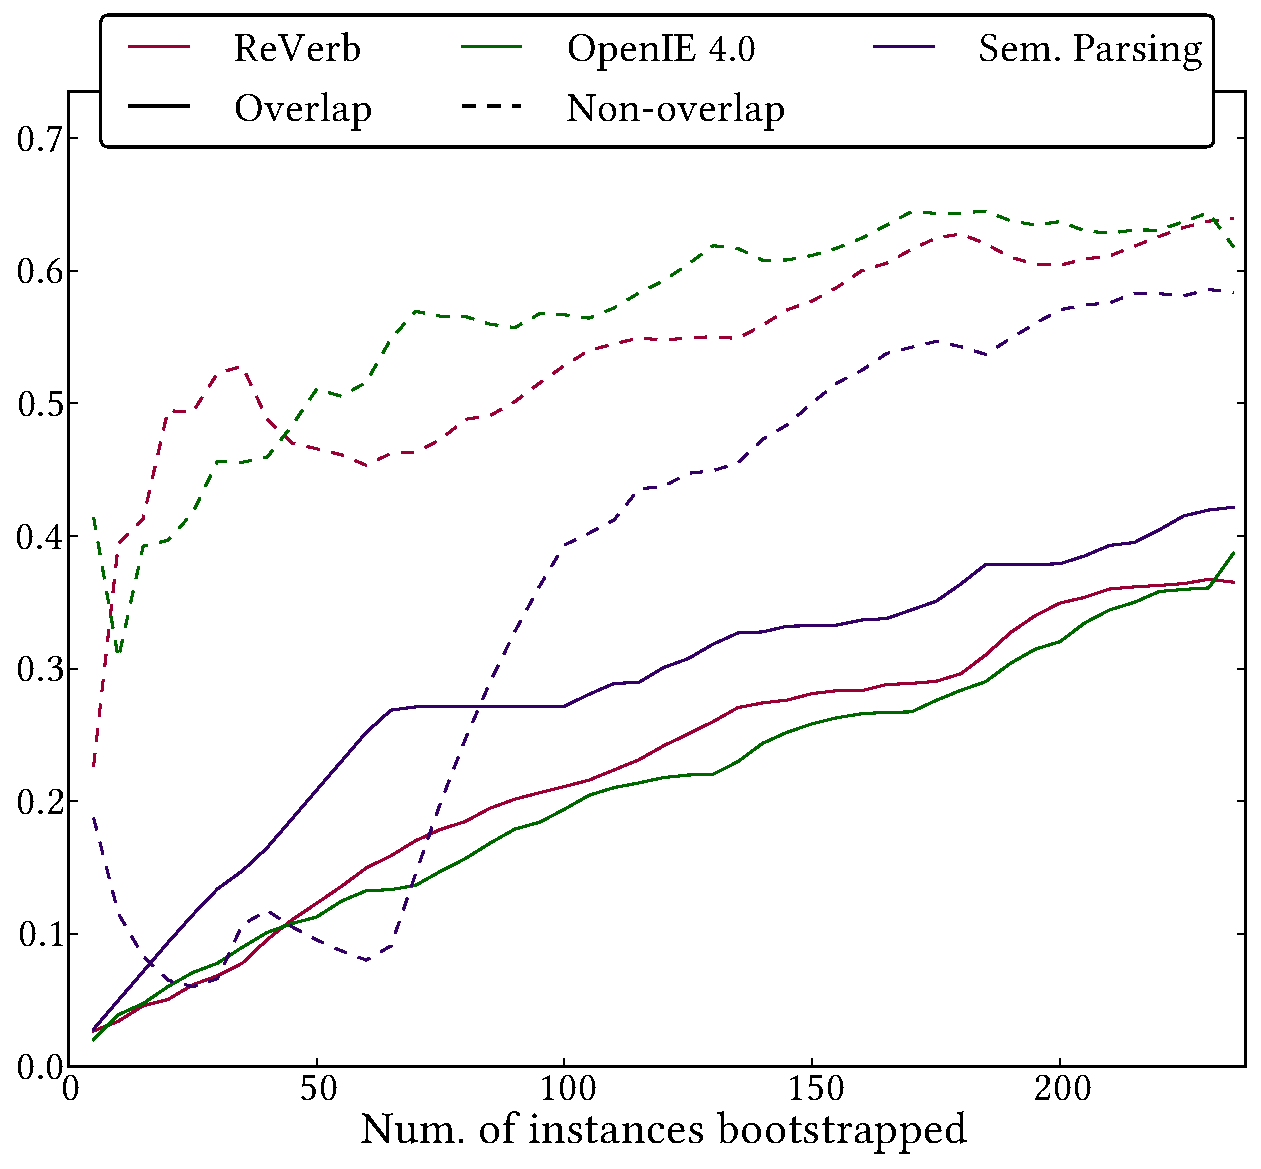
\includegraphics[width=0.45\linewidth]{../data/results/qualitative/object-identification/bootstrapping/hindustani_music/hindustani_singers.pdf}
		 \label{fig:qual-object-bootstrapping-hindustani-singers}
        }%
        \\
        \subfigure[][Ragas]{%
		 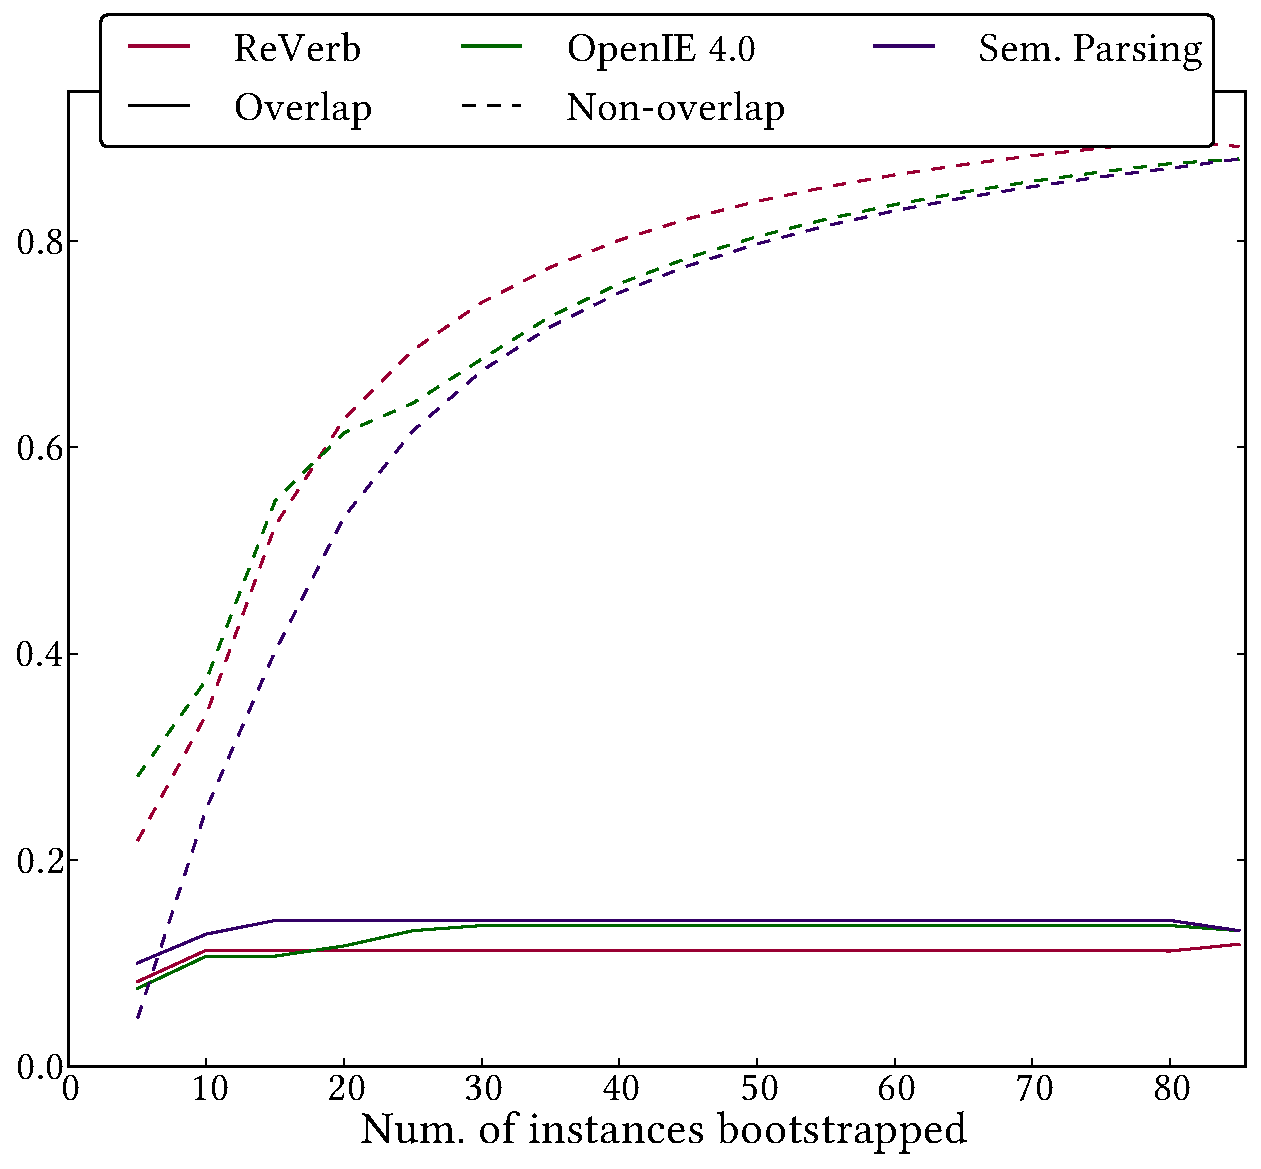
\includegraphics[width=0.45\linewidth]{../data/results/qualitative/object-identification/bootstrapping/hindustani_music/hindustani_ragas.pdf}
		 \label{fig:qual-object-bootstrapping-hindustani-ragas}
        }% 
\end{center}
\caption{Hindustani Results.}
\end{figure}

\subsubsection{Concept identification.}
\subsubsection{Semantic relation extraction.}

\section{Related work}

%TODOs
%KBP and ontology learning in general
%Stephen clark’s semantic network
%Stephen soderland’s OpenIE domain adaptation article and KBP article
%NELL: http://rtw.ml.cmu.edu/rtw/
%http://www.upf.edu/pdi/iula/nuria.bel/#currentresearch

Soderland et al [refs] has proposed a methodology to use the resulting relations from an open information extraction system to populate a domain-specific ontology. One of the main concerns of these approaches is that they require manual engineering to create rules for mapping the relations to ontology.

\section{Conclusions}


\renewcommand\bibname{References}

{\fontsize{9}{10}\selectfont
%\footnotesize
\bibliography{references}
\bibliographystyle{splncs}
}
\end{document}
